\documentclass[
    table,
    12pt,
    oneside, % symmetric pagination
    a4paper,
    %english,
    italian
]{book}
\PassOptionsToPackage{dvipsnames}{xcolor} % colori PDF/A

\usepackage{colorprofiles}
% PDF/A
% validate in https://www.pdf-online.com/osa/validate.aspx
\usepackage[a-1a,mathxmp]{pdfx}[2018/12/22]
%\usepackage{amsmath,amssymb,amsthm} % matematica
\usepackage[T1]{fontenc}
\usepackage[utf8]{inputenc}
\usepackage[italian]{babel}
\usepackage{bookmark}
\usepackage{caption}
\usepackage{chngpage, calc} % centra il frontespizio
\usepackage{csquotes} % gestisce automaticamente i caratteri (")
\usepackage{emptypage} % pagine vuote senza testatina e piede di pagina
\usepackage{epigraph} % per epigrafi
\usepackage{indentfirst} % rientra il primo paragrafo di ogni sezione
\usepackage{graphicx} % immagini
\usepackage[pdfa]{hyperref} % collegamenti ipertestuali
\usepackage{listings} % codici
%\usepackage{microtype} % microtipografia
\usepackage{mparhack,relsize}  % finezze tipografiche
\usepackage{nameref} % visualizza nome dei riferimenti
\usepackage[font=small]{quoting} % citazioni
\usepackage{subfig} % sottofigure, sottotabelle
\usepackage[italian]{varioref} % riferimenti completi della pagina
%\usepackage{booktabs} % tabelle
%\usepackage{tabularx} % tabelle di larghezza prefissata
\usepackage{longtable} % tabelle su più pagine
%\usepackage{ltxtable} % tabelle su più pagine e adattabili in larghezza
\usepackage[toc, acronym, automake]{glossaries}
\usepackage{lmodern}
\usepackage[top=3cm, bottom=2.75cm, right=3cm, left=3.75cm]{geometry} % 1in+17pt+0.6cm
\usepackage{fancyhdr}
\usepackage{lipsum}
\usepackage{setspace}
\usepackage{titlesec}
\usepackage[backend=biber,style=verbose-ibid,hyperref,backref, style=numeric, defernumbers=true]{biblatex} 
% Load variables
\newcommand{\myUni}{Università degli Studi di Padova}
\newcommand{\myDepartment}{Dipartimento di Matematica ``Tullio Levi-Civita''}
\newcommand{\myFaculty}{Corso di Laurea in Informatica}
\newcommand{\myTitle}{Test Automatici con Large Language Model}
\newcommand{\myDegree}{Tesi di Laurea Triennale}
\newcommand{\profTitle}{Prof.}
\newcommand{\myProf}{Ballan Lamberto}
\newcommand{\graduateTitle}{Laureando}
\newcommand{\myName}{Dugo Alberto}
\newcommand{\myStudentID}{2042382}
\newcommand{\myAA}{2023-2024}
\newcommand{\myLocation}{Padova}
\newcommand{\myTime}{Luglio 2024}
% Acronyms
\newacronym[description={\glslink{llmg}{Large Language Model}}]{llm}{LLM}{Large Language Model}
\newacronym[description={\glslink{ideg}{Integrated Development Environment}}]{ide}{IDE}{Integrated Development Environment}
\newacronym[description={\glslink{LoRAg}{Low-Rank Adaptation}}]{lora}{LoRA}{Low-Rank Adaptation}
\newacronym[description={\glslink{llmse}{Assured LLM-Based Software Engineering}}]{llmse}{LLMSE}{Assured LLM-Based Software Engineering}
\newacronym[description={\glslink{peft}{Parameter Efficient Fine-Tuning}}]{peft}{PEFT}{Parameter Efficient Fine-Tuning}
% Glossary
\newglossaryentry{llmg}{
    name=\glslink{llm}{LLM},
    text={Large Language Model},
    sort=llm,
    description={Un Large Language Model (LLM) è un modello capace di generare testi in linguaggio naturale basandosi su modelli statistici.
    Questi modelli acquisiscono una conoscenza linguistica attraverso l'apprendimento di relazioni statistiche durante un processo di addestramento computazionalmente oneroso.}
}

\newglossaryentry{ideg}{
    name=\glslink{ide}{IDE},
    text={Integrated Development Environment},
    sort=ide,
    description={Un Integrated Development Environment (IDE) è un'applicazione software che fornisce servizi per facilitare lo sviluppo di software. Un IDE generalmente comprende un editor di codice sorgente, strumenti di compilazione e debugging e un ambiente per eseguire il software in sviluppo.}
}

\newglossaryentry{LoRAg}{
    name=\glslink{lora}{LoRA},,
    text={Low-Rank Adaptation},
    sort=LoRA,
    description={Approccio di \gls{fine-tuning} il quale permette di costruire diversi modelli per \textit{downstream tasks} i quali ne condividono uno pre-addestrato.}
}

\newglossaryentry{fine-tuning}{
    name={Fine-tuning},
    text={fine-tuning},
    sort=fine-tuning,
    description={Metodologia che permette, attraverso modifiche minimali agli iperparametri di una \textit{neural network}, di adattare un modello ad un nuovo dataset senza doverlo riaddestrare, ottenendo quindi un modello più accurato.}
}

\newglossaryentry{mclearning}{
    name={Machine learning},
    text={machine learning},
    sort=Machine learning,
    description={Branca dell'\textit{intelligenza artificiale} che utilizza metodi statistici per migliorare la performance di un algoritmo nell'identificare pattern nei dati, imparando da questi a svolgere delle funzioni piuttosto che attraverso la programmazione esplicita.}
}

\newglossaryentry{prototipog}{
    name={Prototipo},
    text={prototipo},
    sort=prototipo,
    description={Un prototipo è un esemplare o un modello di un prodotto o di un sistema che viene realizzato antecedentemente al prodotto finale}
}

\newglossaryentry{deeplearning}{
    name={Deep learning},
    text={deep learning},
    sort=Deep learning,
    description={ADD DESCRIPTION.}
}

\newglossaryentry{llmseg}{
    name={Assured LLM-Based Software Engineering},
    text={Assured LLM-Based Software Engineering},
    sort=assured LLM-Based Software Engineering,
    description={ADD DESCRIPTION.}
}
\newglossaryentry{peftg}{
    name={Parameter Efficient Fine-Tuning},
    text={Parameter Efficient Fine-Tuning},
    sort=parameter Efficient Fine-Tuning,
    description={ADD DESCRIPTION.}
}

% Define custom colors
\definecolor{hyperColor}{HTML}{930000}
\definecolor{tableGray}{HTML}{F5F5F7}

% Set line height
\linespread{1.5}

% Custom hyphenation rules
\hyphenation {
    e-sem-pio
    ex-am-ple
}

% Images path
\graphicspath{{img/}}

% Force page color, as some editors set a grayish color as default
\pagecolor{white}

% Better spacing for footnotes
\setlength{\skip\footins}{5mm}
\setlength{\footnotesep}{5mm}

\setlength{\headheight}{14.5pt}
\addtolength{\topmargin}{-2.45pt}

% Listings setup
\lstset{
    language=[LaTeX]Tex,%C++,
    keywordstyle=\color{RoyalBlue}, %\bfseries,
    basicstyle=\small\ttfamily,
    %identifierstyle=\color{NavyBlue},
    commentstyle=\color{Green}\ttfamily,
    stringstyle=\rmfamily,
    numbers=none, %left,%
    numberstyle=\scriptsize, %\tiny
    stepnumber=5,
    numbersep=8pt,
    showstringspaces=false,
    breaklines=true,
    frameround=ftff,
    frame=single
}

% Add a subscript G to a glossary entry
\newcommand{\glox}{\textsubscript{\textbf{\textit{G }}}}

% If the subscript G is followed by a punctuation character, or anything else, you need to use \gloxspacing to prevent rendering issues, where the characters collide. Example in Chapter 7
\newcommand{\gloxspacing}{\hspace{-0.3em}}

% Improvements the paragraph command
\titleformat{\paragraph}
{\normalfont\normalsize\bfseries}{\theparagraph}{1em}{}
\titlespacing*{\paragraph}
{0pt}{3.25ex plus 1ex minus .2ex}{1.5ex plus .2ex}

% Define use case environment
\newcounter{usecasecounter} % define a counter
\setcounter{usecasecounter}{0} % set the counter to some initial value
% Parameters
% #1: ID
% #2: Nome
\newenvironment{usecase}[2]{
    \renewcommand{\theusecasecounter}{\usecasename #1}  % this is where the display of the counter is overwritten/modified
    \refstepcounter{usecasecounter} % increment counter
    \vspace{2em}
    \par \noindent % start new paragraph
    {\normalsize \textbf{\usecasename #1: #2}} % display the title before the content of the environment is displayed
    \vspace{.5em}
}{
    \medskip
}
\newcommand{\usecasename}{UC}
\newcommand{\usecaseactors}[1]{\textbf{\\Attori Principali:} #1}
\newcommand{\usecasepre}[1]{\textbf{\\Precondizioni:} #1}
\newcommand{\usecasedesc}[1]{\textbf{\\Descrizione:} #1}
\newcommand{\usecasepost}[1]{\textbf{\\Postcondizioni:} #1}
\newcommand{\usecasealt}[1]{\textbf{\\Scenario Alternativo:} #1}

% Define risks environment
\newcounter{riskcounter} % define a counter
\setcounter{riskcounter}{0} % set the counter to some initial value
% Parameters
% #1: Title
\newenvironment{risk}[1]{
    \refstepcounter{riskcounter} % increment counter
    \par \noindent % start new paragraph
    \textbf{\arabic{riskcounter}. #1} % display the title before the content of the environment is displayed
}{
    \par\medskip
}
\newcommand{\riskname}{Rischio}
\newcommand{\riskdescription}[1]{\textbf{\\Descrizione:} #1.}
\newcommand{\risksolution}[1]{\textbf{\\Soluzione:} #1.}

% Apply fancy styling to pages
\pagestyle{fancy}
\fancyhf{}
\fancyhead[L]{\leftmark} % Places Chapter N. Chatper title on the top left
\fancyfoot[C]{\thepage} % Page number in the center of the footer

% Adds a blank page while increasing the page number
\newcommand\blankpage{ 
    \clearpage
    \begingroup
      \null
      \thispagestyle{empty}
      \hypersetup{pageanchor=false}
      \clearpage
    \endgroup
}

% Increase page numbering
\newcommand\increasepagenumbering{
    \addtocounter{page}{+1}
}

% Make glossaries and bibliography
\makeglossaries
\bibliography{references/bibliography}
\defbibheading{bibliography} {
    \cleardoublepage
    \phantomsection
    \addcontentsline{toc}{chapter}{\bibname}
    \chapter*{\bibname\markboth{\bibname}{\bibname}}
}
\glsaddall

% Set up hyperlinks
\hypersetup{
    colorlinks=true,
    linktocpage=true,
    pdfstartpage=1,
    pdfstartview=,
    breaklinks=true,
    pdfpagemode=UseNone,
    pageanchor=true,
    pdfpagemode=UseOutlines,
    plainpages=false,
    bookmarksnumbered,
    bookmarksopen=true,
    bookmarksopenlevel=1,
    hypertexnames=true,
    pdfhighlight=/O,
    allcolors = hyperColor
}

% Set up captions
\captionsetup{
    tableposition=top,
    figureposition=bottom,
    font=small,
    format=hang,
    labelfont=bf
}

\date{}
\hypersetup{pdfstartview=}
\begin{document}
    %\layout
    \frontmatter
    \begin{titlepage}
    \begin{center}
        \begin{Large}
            \textbf{\myUni}\\
        \end{Large}

        \vspace{5pt}

        \begin{large}
            \textsc{\myDepartment}\\
        \end{large}

        \vspace{5pt}

        \begin{large}
            \textsc{\myFaculty}\\
        \end{large}

        \vspace{25pt}
        
        \begin{figure}[htbp]
            \centering
            
\includegraphics[alt={Emblema dell'Università degli Studi di Padova}, height=6cm]{img/logo_unipd.jpeg}
        \end{figure}

        
        \begin{Large}
            \textbf{\myTitle}\\
        \end{Large}

        \vspace{5pt}

        \begin{large}
            \textit{\myDegree}\\
        \end{large}

        \vspace{50pt}
        
        \begin{normalsize}
            \begin{flushleft}
                \textit{Relatore}\\
                \profTitle\ \myProf
            \end{flushleft}

            \vspace{-48pt}
            
            \begin{flushright}
                \textit{\graduateTitle}\\
                \myName\\
                Matricola \myStudentID
            \end{flushright}
        \end{normalsize}

        \vspace*{\fill}
        
        \line(1, 0){338} \\
        \begin{normalsize}
            \textsc{Anno Accademico \myAA}
        \end{normalsize}
    \end{center}
\end{titlepage}

    \increasepagenumbering % increase the page numbrering by 1, in order to cout the frontispiece
    \clearpage
\phantomsection
\thispagestyle{empty}
\hfill
\vfill

{\small\noindent\textcopyright\ \myName, \myTime. Tutti i diritti riservati. \myDegree: ``\textit{\myTitle}'', \myUni, \myDepartment.}
    \cleardoublepage
\phantomsection
\pdfbookmark{Ringraziamenti}{Ringraziamenti}

%\begin{flushright}{
    %\slshape
   %``No matter how much they want it, I want it more''} \\
    %\medskip
    %--- Lewis Hamilton
%\end{flushright}

\begingroup
\let\clearpage\relax
\let\cleardoublepage\relax
\let\cleardoublepage\relax

\chapter*{Ringraziamenti}

\noindent %Desidero esprimere la mia gratitudine al professor \myProf, mio relatore, per l'aiuto e il sostegno che mi ha dato durante la stesura dell'elaborato.

\noindent %rigraziamenti2\\
\noindent %ringraziamenti3

\vspace{0.75cm}

\noindent{\myLocation, \myTime}
\hfill \textit{\myName}

\endgroup

    \cleardoublepage
\phantomsection
\pdfbookmark{Compendio}{Compendio}
\begingroup
\let\clearpage\relax
\let\cleardoublepage\relax
\chapter*{Abstract}
Il presente documento illustra l'attività di stage svolta dal laureando Alberto Dugo presso l'azienda Zucchetti Spa.
\\Durante il periodo di stage, della durata di 320 ore, vi è stata l'opportunità di approfondire le conoscenze in ambito \gls{mclearning}\glox.
In particolare era richiesto lo studio e l'implementazione di test automatici derivanti direttamente dal codice, sfruttando le abilità dei sistemi di intelligenza artificiale ed in particolare del \gls{llm}\glox\gloxspacing.
Vi è stato inoltre la possibilità di fare \gls{fine-tuning}\glox dei modelli \gls{llm} attraverso il metodo \gls{lora}\glox e quantizzare i modelli stessi in modo da renderli più efficienti.
\endgroup
\vfill

    \blankpage % example of a blank page, that also increases the page couter by 1
    \cleardoublepage
\pdfbookmark{\contentsname}{tableofcontents}
\setcounter{secnumdepth}{5}  % Numbering depth for sections
\setcounter{tocdepth}{5}     
% Depth of entries in the table of contents

\tableofcontents
%\markboth{\contentsname}{\contentsname}
\clearpage

\begingroup
    \let\clearpage\relax
    \let\cleardoublepage\relax
    \let\cleardoublepage\relax

    % Figures list
    \phantomsection
    \pdfbookmark{\listfigurename}{lof}
    \listoffigures

    \vspace*{8ex}

    % Tables list
    \phantomsection
    \pdfbookmark{\listtablename}{lot}
    \listoftables

    \vspace*{8ex}
\endgroup

\cleardoublepage
    

    \mainmatter
    \chapter{Introduzione}
\label{chap:introduzione}



%Introduzione al contesto applicativo.

%Lorem Figure \ref{fig:entanglement}

%Esempio di utilizzo di un termine nel glossario \gls{api}.

%Esempio di citazione nel piè di pagina citazione\footcite{womak:lean-thinking}

%\lipsum[1-2]

\section{L'azienda}
\begin{figure}[h!]
    \centering
    
\includegraphics[alt={Testo alternativo dell'immagine}, width=0.7\columnwidth]{img/logoZucchetti.jpeg}
    \caption{logo di Zucchetti}
    \label{fig:entanglement}
\end{figure}
Zucchetti S.p.a. è la prima software house in Italia per fatturato, opera nel settore dell'\textit{Information Technology}, ed è stata fondata nel 1978 da Fabrizio Bernini a Lodi. 
L'azienda è specializzata nella realizzazione di software gestionali per pianificazione delle risorse d'impresa, soluzioni per il controllo degli accessi e sistemi di automazione industriale. 
Al giorno d'oggi Zucchetti oltre ad avere sedi in tutta Italia è presente anche in 50 paesi esteri, tra cui Cina, Germania, USA e Svizzera e conta più di 8.000 dipendenti e più di 1650 \textit{partner}.

\section{Il progetto}
Lo \textit{stage} si è svolto presso l'azienda Zucchetti, con sede a Padova. Il progetto di \textit{stage} ha previsto la ricerca e lo sviluppo di test automatici derivanti direttamente dal codice e dalla documentazione, sfruttando le abilità dei sistemi di \textit{intelligenza artificiale} ed in particolare dei \glspl{llmg}.
Lo \textit{stage} è stato diviso in due macroperiodi di quattro settimane ciascuno. Nel primo periodo ho analizzato, attraverso lo studio di paper accademici e documentazioni, le tecniche di \textit{testing} che sfruttano \glspl{llmg}. Successivamente ho implementato un \gls{prototipog} di generatore di test automatici in \textit{Python} che usufruisce di un modello basato su \textit{natural language processing}. Nella seconda parte del primo periodo ho decorato il codice attraverso commenti e ho generato \textit{test}. I risultati di questi sono stati poi confrontati con quelli ottenuti dalla prima parte di periodo. Nel secondo periodo invece ho eseguito \gls{fine-tuning} dei modelli \glspl{llm} con il metodo \gls{lora}, per poi confrontare i risultati ottenuti con quelli nel primo periodo.
È stato inoltre richiesto lo studio di tecniche di \textit{quantizzazione} per ridurre la dimensione dei modelli \glspl{llm} e la loro complessità computazionale.
\section{Organizzazione del testo}
\begin{description}
    \item[{\hyperref[chap:processi-metodologie]{Il secondo capitolo}}] descrive i processi e le metodologie utilizzate durante lo \textit{stage}. In particolare si approfondiranno i processi di sviluppo \textit{software} e gli strumenti utilizzati per fare ciò.
    
    \item[{\hyperref[chap:descrizione-stage-1]{Il terzo capitolo}}] si propone di delineare il dominio applicativo del progetto, mediante un'analisi dettagliata del tema accompagnata da esempi pratici di utilizzo. 
    Inoltre, si provvederà a fornire una descrizione esaustiva del funzionamento di \textit{Assured LLMS}. 
    In questa sezione, sarà altresì redatta una lista esaustiva di rischi, requisiti e obiettivi del progetto. 
    Successivamente, si procederà con la descrizione del prodotto sviluppato, che includerà \textit{script} e \textit{benchmarks}. 

    \item[{\hyperref[chap:descrizione-stage-2]{Il quarto capitolo}}] descrive il processo di applicazione di \gls{lora} e le possibili ottimizzazioni, andando ad approfondire le tecniche utilizzate durante il processo.

    \item[{\hyperref[chap:conclusioni]{Il quinto capitolo}}] concluderà il documento, presentando una valutazione retrospettiva personale dell'esperienza di \textit{stage} e delle conoscenze acquisite.
    
\end{description}

In seguito si possono trovare le convenzioni tipografiche utilizzate per la stesura del documento:
\begin{itemize}
	\item gli acronimi, le abbreviazioni e i termini ambigui o di uso non comune menzionati vengono definiti nel glossario, situato alla fine del presente documento;
	\item per la prima occorrenza dei termini riportati nel glossario viene utilizzata la seguente nomenclatura: \textit{parola}\glox\gloxspacing;
	\item i termini in lingua straniera o facenti parti del gergo tecnico sono evidenziati con il carattere \textit{corsivo}.
\end{itemize}

\newpage
    \chapter{Processi e metodologie}
\label{chap:processi-metodologie}

Lorem ipsum dolor sit amet, consectetuer adipiscing elit. Aenean commodo ligula eget dolor. Aenean massa. Cum sociis natoque\footnote{\cite{site:agile-manifesto}} penatibus et magnis dis parturient montes, nascetur ridiculus mus. Donec quam felis, ultricies nec\footnote{\cite{article:spooky}}, pellentesque eu, pretium quis, sem.

\begin{figure}[h]
    \centering
    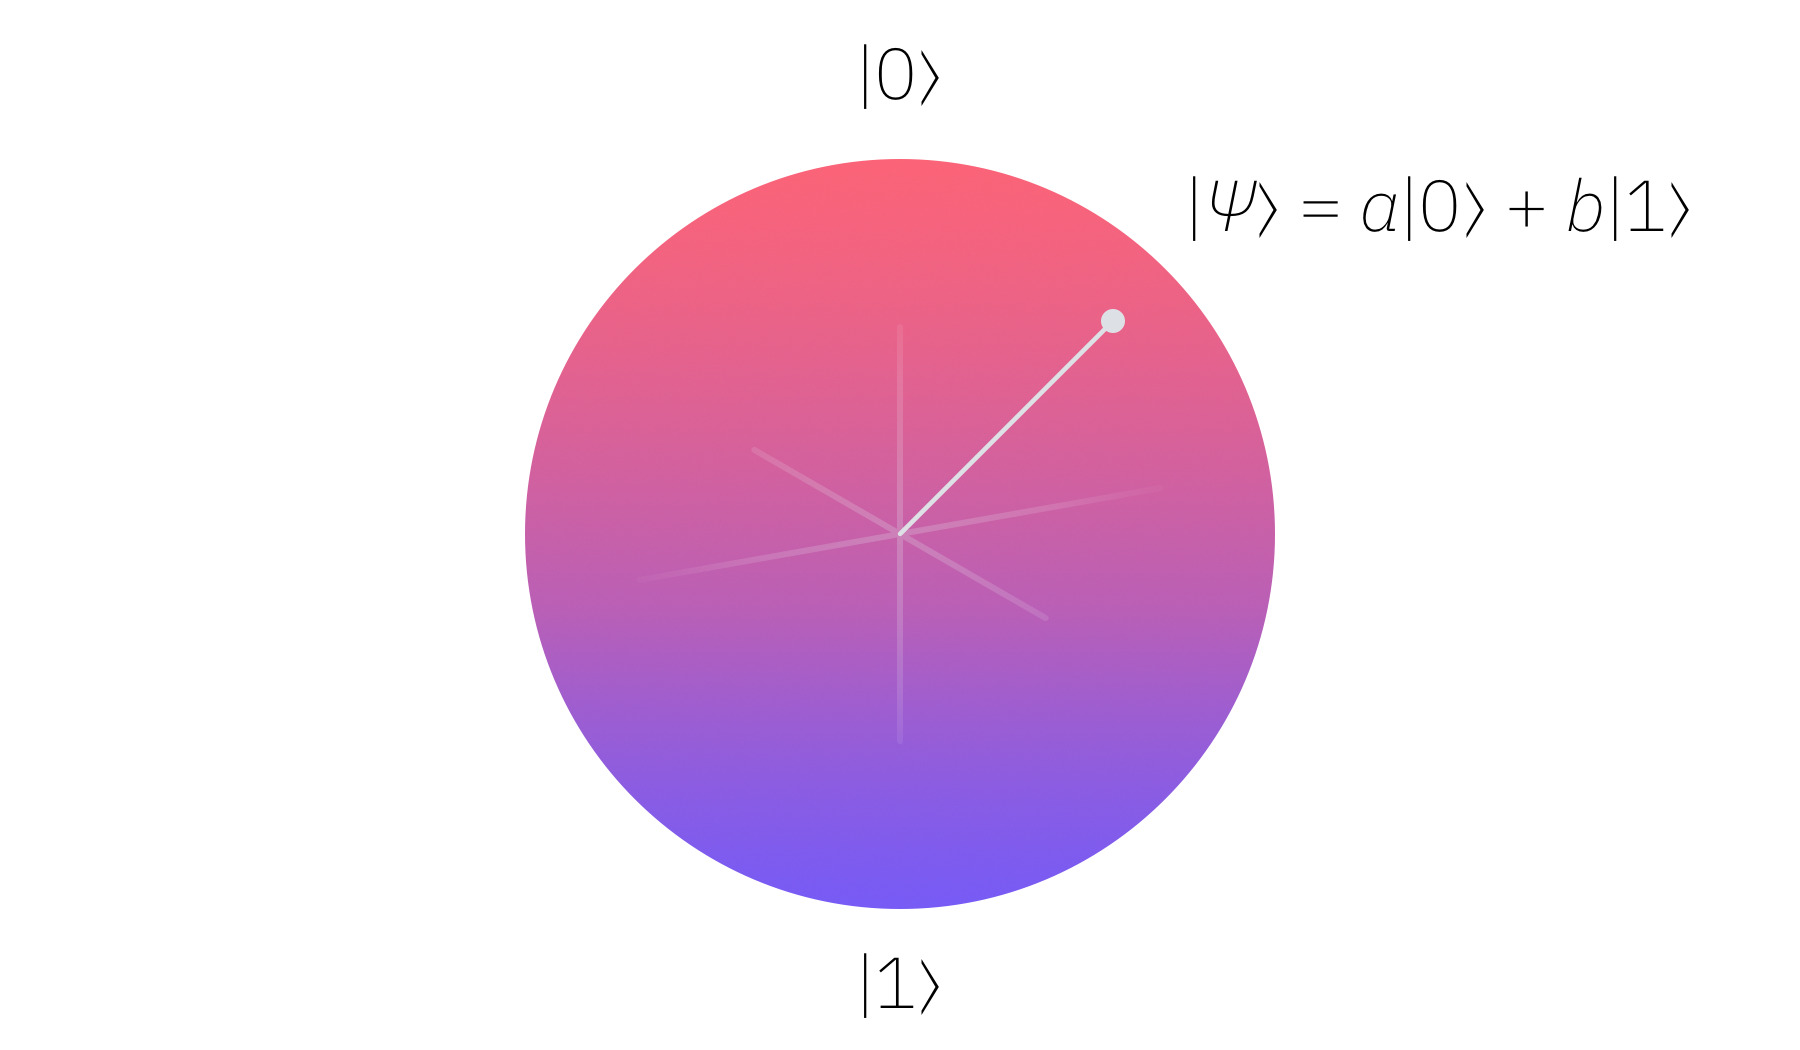
\includegraphics[alt={Testo alternativo dell'immagine}, height=5cm]{img/qubit.jpeg}
    \caption{Lorem}
    \label{fig:qubit}
\end{figure}
\lipsum[1]

\section{Processo sviluppo prodotto}
\lipsum[1-2]

\newpage
    \chapter{Test automatici generati da LLM}
\label{chap:descrizione-stage-1}
\section{Analisi del dominio applicativo}
Durante la fase di analisi del dominio applicativo si è proceduto a delineare il contesto in cui il progetto si colloca, analizzando il tema e fornendo esempi pratici di utilizzo. Inoltre, si è provveduto a fornire una descrizione esaustiva del funzionamento di \gls{llmse}\glox, tipologia di \gls{llmg} che sta alla base del funzionamento del prodotto.
    \subsection{Analisi del tema}
    Il tema del progetto riguarda la realizzazione di \textit{test} automatici per il codice sorgente, ponendosi come obiettivo la semplificazione del processo di \textit{testing} affidato ai programmatori attraverso l'utilizzo di \glspl{llmg}.
    In particolare, il progetto consiste in uno \textit{script} nel quale si andrà ad estrarre i metodi e le classi da testare cercando le relazioni tra di essi, in seguito verrà spigato dettagliatamete come è stato eseguito questo passaggio.
    Lo \textit{script} in questione dovrà quindi utilizzare predizioni dettate dal \gls{llmg} per generare \textit{test} automatici. Quest'ultimi verranno poi eseguiti e i risultati verranno riportati in grafici per una migliore comprensione.  
    %dopodichè sarà necessario applicare dei filtri per migliorare i risultati ottenuti.
    %Questi filtri sono necessari in quanto, se non applicati, il modello potrebbe generare \textit{test} non validi.

    %descrive il dominio del problema da affrontare:
    %la porzione del mondo reale, rilevante per il sistema\\
    %-> Su cui si devono mantenere informazioni\\
    %-> Concuisideve interagire

    %Dopo la generazione di \textit{test} e il \textit{filtering} di essi, si dovranno quindi salvare nei corrispettivi \textit{file ad hoc}.

    \subsection{Esempi di utilizzo}
    Negli ultimi anni si è registrato un aumento significativo nell'adozione dei \glspl{llmg} per la generazione di testo, con una crescita esponenziale soprattutto nel settore tecnologico.
    In questa sezione esamineremo il loro utilizzo in ambito di \textit{testing} del codice sorgente.
    In particolare è noto che l'utilizzo di \glspl{llmg} per la generazione di \textit{test} automatici è in grado di ridurre i tempi di \textit{testing} del codice sorgente e migliorare la qualità del codice stesso\cite{article:Alshahwan2024AutomatedUT}.
    La capacità di generare test aumenta inoltre la verificabilità di non regressione del codice, in questo momento però non si è in grado di verificare la presenza di \textit{bug} nel codice senza l'aiuto del programmatore, è chiaro quindi che gli \glspl{llm} in questo periodo storico riescano a fornire solamente un supporto ai programmatori anzichè sostituirli.
        %Automatizzazione dei test attraverso llm in modo da aumentare il test coverage dei corner case
        %ridurre bug 
        %ridurre tempo di sviluppo dei test 
    \subsection{\textit{Assured LLMSE}}
    Negli ultimi anni nell'ambito del Software Engineering si è assistito ad una crescita elevata nell'utilizzo dell'intelligenza artificiale volto alla ricerca di agevolare il programmatore durante lo sviluppo di software.
    Proprio in quest'ambito ci riferiamo a \gls{llmse} per descrivere una qualsiasi tipo di applicazione nella quale il prodotto o i processi software si basano sull'utilizzo di \gls{llm}\cite{article:Alshahwan2024AssuredLS}.
    Alla base di questo progetto troviamo quindi un massiccio uso degli \glspl{llm} ed in particolare il progetto in sè vuole fornire uno strumento ai programmatori, il quale agevola la scrittura dei \textit{test} attraverso l'utilizzo di \gls{llm}.
    \begin{figure}[!h]
        \centering        
        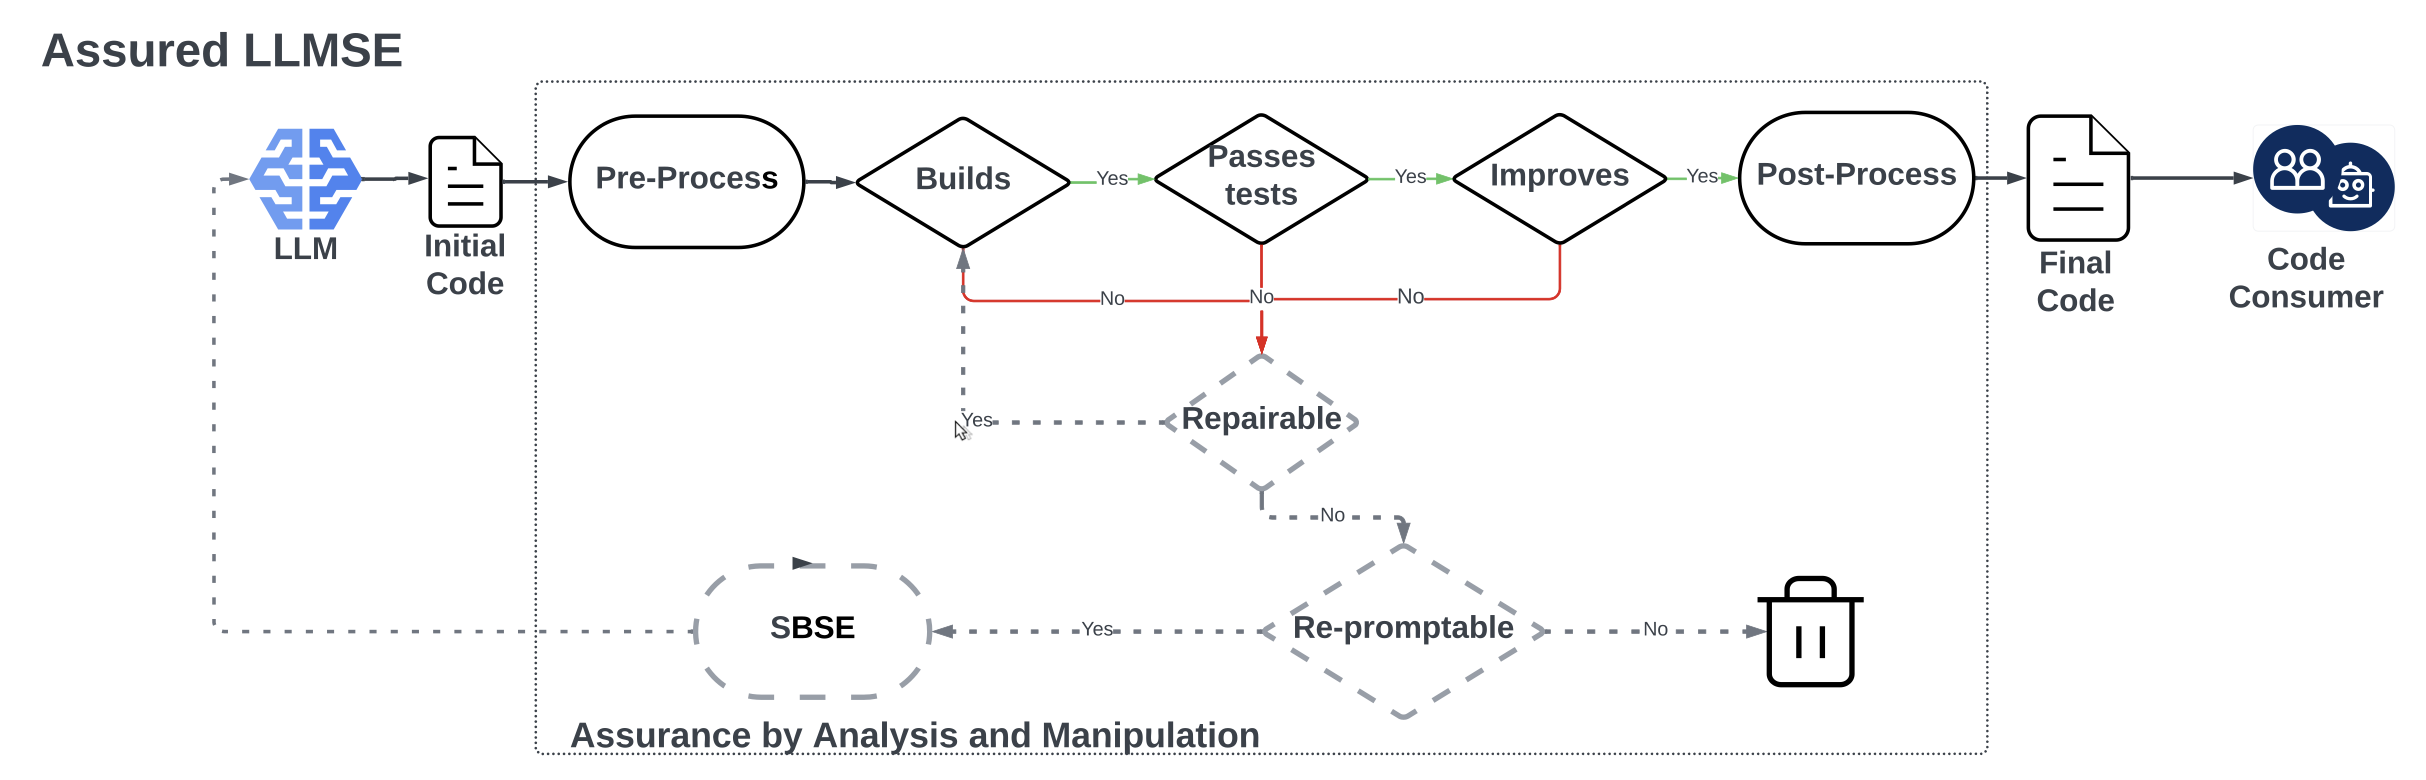
\includegraphics[width=14.5cm]{img/LLMSE.png}
        \caption{Architettura \gls{llmse}\cite{article:Alshahwan2024AssuredLS}}
    \end{figure}
  \\Lo scopo degli \gls{llmse} è quello di applicare una serie di filtri semantici al codice generato in modo tale da poter fornire delle garanzie, come ad esempio l'assenza di allucinazioni.
    Come infatti è visibile in figura 3.1 dopo la generazione della risposta da parte del \gls{llmg} questa viene pre-processata, quindi si eliminano i vari commenti non soggetti a \textit{test}, e si estrae solamente il codice.
    Dopodichè vengono applicati svariati filtri, tra cui la capacità di essere nello stato di \textit{build}, di essere in stato di accettazione, quindi che l'asserzione di esso sia \textit{true} ed inoltre che sia in grado di aumentare la \textit{code coverage}.
    Possiamo notare che se anche solo uno di questi filtri condizionali non desse risultato positivo l'intero \textit{test} affronterebbe altri filtri condizionali i quali potrebbero portare alla sua eliminazione.
    Le condizionalità dovute ad un possibile fallimento di una condizione sono esplicitate nella procedura in seguito:
    \begin{lstlisting}[language=Python]
        def filtering(self, facadeFilter):
            if test.repairable():
                test.repair()
                return facadeFilter.filters(test)
            elif test.re_prompable():
                prompt = test.re_prompt()
                return self.ask(prompt)
            else:
                return test.discard()
    \end{lstlisting}
    
    Nel flusso procedurale, un test scartato viene immediatamente sottoposto al filtro \textit{''Repairable''}. In questo scenario, se è possibile riparare il codice rapidamente senza dover riformulare l'intero prompt, allora viene effettuata la riparazione e il test riprende il processo di filtraggio. Altrimenti, il test procede con i filtri successivi.
    Nel caso in cui il \textit{Re-prompt} sia possibile, permettendo così di ottimizzare il prompt mediante una riformulazione, il \textit{test} può avanzare alla fase successiva, altrimenti, viene eliminato definitivamente.
    Il \textit{re-prompting} avviene attraverso \textit{Search-based software engineering (SBSE)} che è una tipologia di ottimizzazione del prompt la quale si basa su un algoritmi genetici, la rigenerazione del prompt permette quindi di ricominciare l'interno processo.
    I filtri in questione, nel caso in cui il \textit{test} non fosse approvato, sono filtri opzionali, vedremo in seguito che questi vengono omessi durante il processo di sviluppo per ovviare ai costi onerosi derivati.
    Il codice quindi che supera tutti i filtri è un codice che soddisfa i requisiti e può essere passato ad un consumatore, il quale potrebbe essere ad esempio un umano o un altro tool.\newline
        %X cosa sono 
        %X come funzionano 
        %X perchè sono importanti per il progetto 
    \subsubsection{\textit{Offline} ed \textit{Online} LLMSE}
        %distinzione tra off e online
        È importante distinguere \textit{Online} e \textit{Offline} \gls{llmse}, in quanto il primo necessita della risposta dell'\gls{llm} in \textit{real time}, mentre il secondo non pone vincoli temporali.
        Nel contesto dell'\textit{Online} \gls{llmse}, facciamo riferimento, ad esempio, alle applicazioni di completamento automatico del codice, come \textit{CoPilot}. Qui, la tempestività della risposta del modello è fondamentale per l'esperienza utente.
        D'altra parte, l'\textit{Offline} \gls{llmse} si riferisce a processi in cui non è necessaria una risposta immediata. Nei casi di \textit{Offline} \gls{llmse}, se il tempo di generazione della risposta dovesse variare, ciò non influirebbe sul funzionamento dell'applicazione stessa. Nel caso del mio progetto, andrò ad utilizzare \textit{Offline} \gls{llmse} poichè quest'utlimi permettono
        di poter applicare i filtri che abbiamo precedentemente descritto senza dover preoccuparsi del tempo di risposta.
    \subsubsection{Future applicazioni e miglioramenti} 
        Per quanto riguarda le future applicazioni,
        il miglioramento dei filtri è sicuramente uno dei maggiori potenziali di sviluppo, in questo modo si riuscirebbe ad ottenere risultati migliori e più adatti alle esigenze.
        Non solo il miglioramento dei filtri, ma anche l'utilizzo di \textit{Genetic Improvement} per migliorare il \textit{prompt} e \textit{Methauristic algorithm} per migliorare le soluzioni candidate potrebbero portare a risultati migliori.
        Il miglioramento del \textit{prompt} è un'area di ricerca molto promettente, in quanto un \textit{prompt} ben formulato è in grado di guidare l'\gls{llm} verso la generazione di test più accurati e corretti.
        \textit{In-learning context} è un'altra area di ricerca che potrebbe portare a risultati significativi. In questo contesto, l'\gls{llm} è in grado di apprendere dai risultati ottenuti e di migliorare le proprie prestazioni nel tempo.
        Possiamo quindi ipotizzare che ponendo maggiore attenzione a formulare il prompt in modo più accurato, sfruttando algoritmi genetici e applicando le tecniche di \textit{prompt engineering}, si possa ottenere un \gls{llm} più performante e in grado di generare test più accurati e corretti.
        %future applicazioni (?)
        %   -> migliorare filtri
        %   -> Genetic Improvement per migliorare prompt e Methauristic algorithm per migliorare candidate solutions
        %   -> prompt engineering
        %   -> in-learning context
\section{Analisi dei requisiti}
    \subsection{Analisi preventiva dei rischi}
    Durante la fase di analisi dei rischi sono stati individuate le possibili criticità che potranno essere riscontrate.
    Si è quindi proceduto a elaborare delle possibili soluzioni per far fronte a tali rischi.

    \begin{risk}{Mancanza di materiale informativo}
        \riskdescription{Trattandosi di una novità nel settore e in fase di crescita, la possibile assenza di materiale informativo relativo all'argomento stesso potrebbe rallentare il processo di apprendimento}
        \risksolution{coinvolgimento del responsabile a capo del progetto relativo}
        \label{risk:data-absence} 
    \end{risk}

    \subsection{Requisiti e obiettivi}

    \begin{center}
        \rowcolors{1}{}{tableGray}
        \begin{longtable}{|p{2.25cm}|p{7.75cm}|p{2.25cm}|}
        \hline
        \multicolumn{1}{|c|}{\textbf{Obiettivo}} & \multicolumn{1}{c|}{\textbf{Descrizione}}\\ 
        \hline 
        \endfirsthead
        \multicolumn{3}{c}%
        {{\bfseries \tablename\ \thetable{} -- Continuo della tabella}}\\
        \hline
        \multicolumn{1}{|c|}{\textbf{Obiettivo}} & \multicolumn{1}{c|}{Descrizione}\\ \hline 
        \endhead
        \hline
        \multicolumn{3}{|r|}{{Continua nella prossima pagina...}}\\
        \hline
        \endfoot
        \endlastfoot 
        OB 1 & Realizzazione di smoke \textit{test} in Python generati da codice reale. \\
        \hline
        OB 2 & Realizzazione di decorazioni assert per funzioni. \\
        \hline
        OB 3 & Realizzazione di \textit{test} a partire da codice commentato. \\
        \hiderowcolors
        \caption{Requisiti primo macroperiodo.}
        \label{tab:requisiti_obbiettivi}
        \end{longtable}
    \end{center}


\newpage
\section{Sviluppo del prodotto}
    A seguito dello studio del dominio e delle opportunità vi è stata la progettazione e lo sviluppo del prodotto. 
    Questo capitolo si propone di offrire un'esauriente panoramica sul processo di sviluppo del prodotto, esaminando in dettaglio le tappe fondamentali che ho affrontato.
    In particolare, ci concentreremo sull'analisi dello \textit{script} realizzato per l'estrazione e la generazione dei \textit{test}, una fase cruciale che ha richiesto un'accurata progettazione e implementazione.
    Saranno descritti poi i risultati ottenuti attraverso un'analisi dettagliata, evidenziando le sfide superate e i successi raggiunti nel corso del processo di sviluppo.
    
    \subsection{\textit{Script}}
    Lo \textit{script} generato permette di fare il parsing di un intero progetto salvando dati chiave all’interno di un \textit{database} \textit{SQlite}. 
    Questo procedimento permette all'\gls{llm} di riuscire a trovare le relazioni all’interno dei dati. 
    Dopo il processo di \textit{parsing} è possibile generare i \textit{test} attraverso l'\gls{llm}. Utilizzando infatti i comandi –-genTestClass e --genTestMethod è possibile generare i \textit{test} per una classe o per un metodo specifico.
    Il seguente \textit{script} può quindi essere azionato attraverso linea di comando utilizzando vari comandi:
    \begin{itemize}
        \item “python3 –-parseProj nameProject” : si farà solamente il parsing di tutti i file all’interno del progetto.
        \item “python3 –-genTestClass Class\_Name Method\_Name: attraverso questo comando è possibile generare i \textit{test} per un particolare metodo all’interno della classe specificata.
        \item “python3 --genTestMethod Class\_Name: attraverso questo comando è possibile generare i \textit{test} per la singola classe.
    \end{itemize}
    In figura 3.2 viene descritto come sono stati realizzati.\\
    \begin{figure}[!h]
        \centering        
        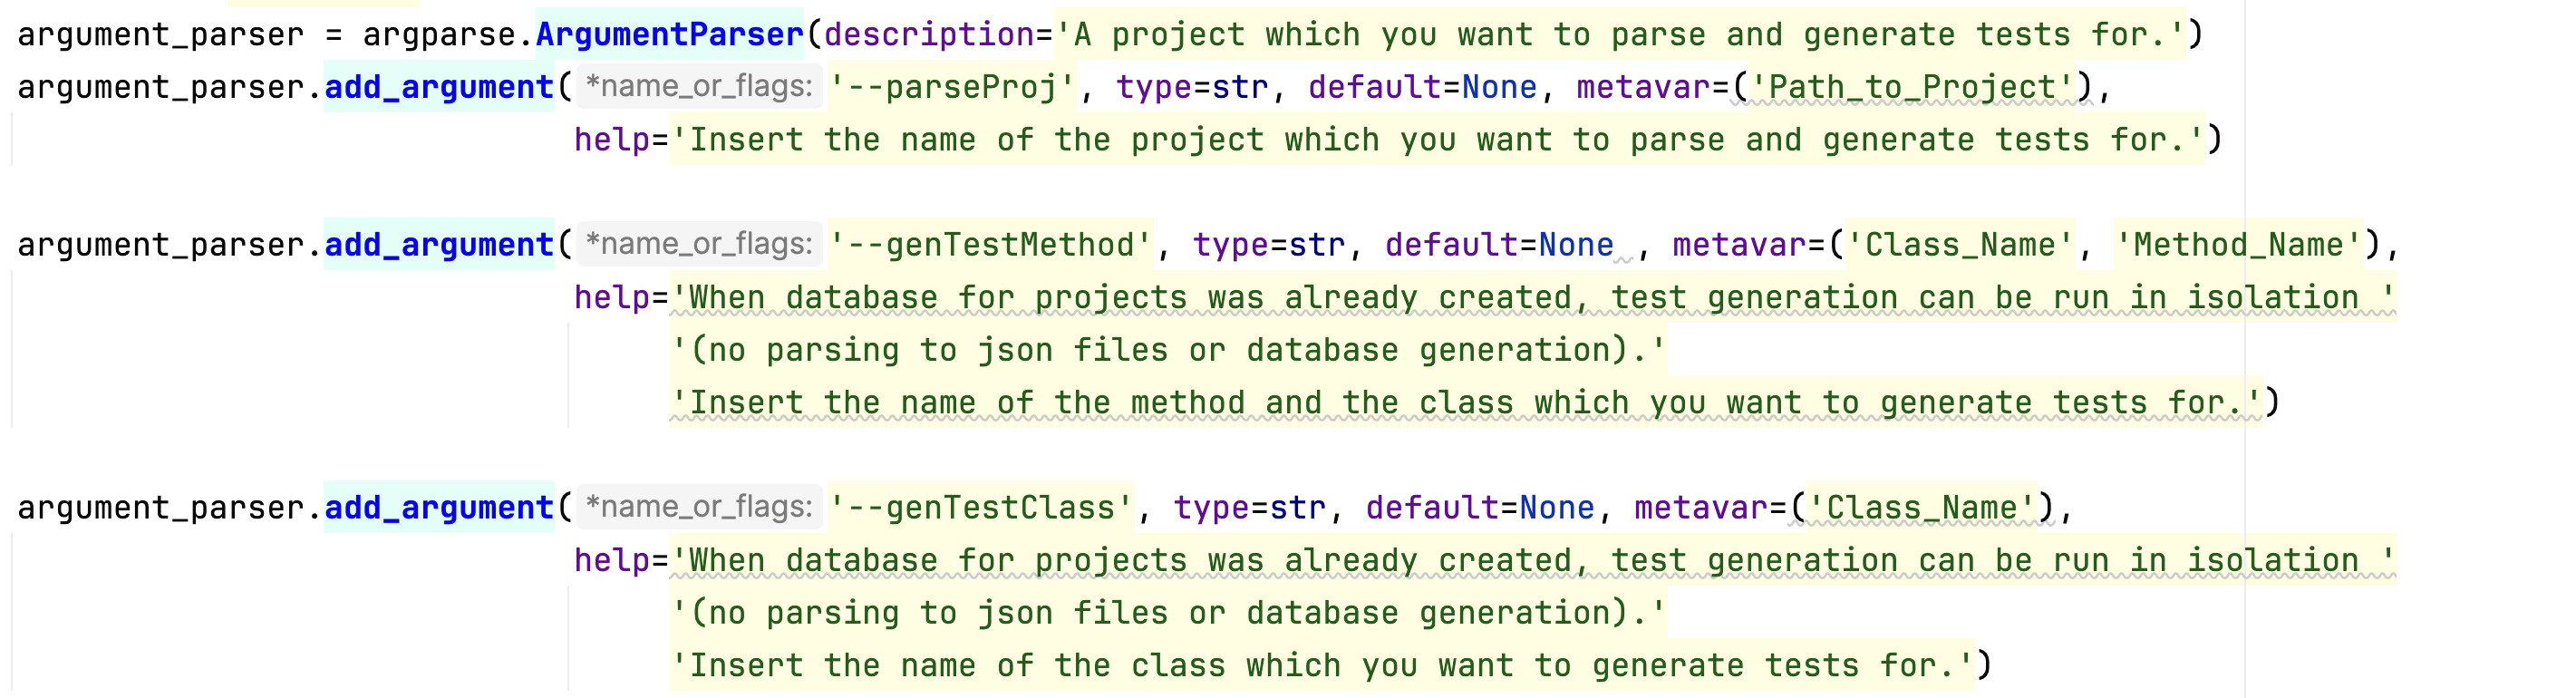
\includegraphics[width=14.5cm]{img/script argument.png}
        \caption{Comandi \textit{script}}
    \end{figure}\newline

    \subsubsection{\textit{Parsing del linguaggio}}
    Inizialmente, lo \textit{script} richiede di eseguire l'analisi del progetto, focalizzandosi principalmente sull'estrazione di ogni file con estensione \textit{.py}
    e sulla categorizzazione di ciascuna istruzione all'interno di un nodo dell'albero di parsing. Tale processo è indispensabile poichè altrimenti sarebbe 
    impossibile delineare le relazioni esistenti tra i vari metodi e le classi.
    Una volta estratte e categorizzate tutte le istruzioni all'interno dei nodi dell'albero, vengono recuperate le firme dei metodi e delle classi. 
    Queste informazioni vengono quindi archiviate nel database SQLite insieme ai \textit{related method}, ovvero i metodi chiamati all'interno di altri metodi. 
    Tale approccio ci consente di identificare le relazioni intrinseche presenti nel progetto e di ottenere risultati più accurati.
    L'idea di base può essere confermata attraverso i dati in figura 3.3.
    \begin{figure}[!h]
        \centering        
        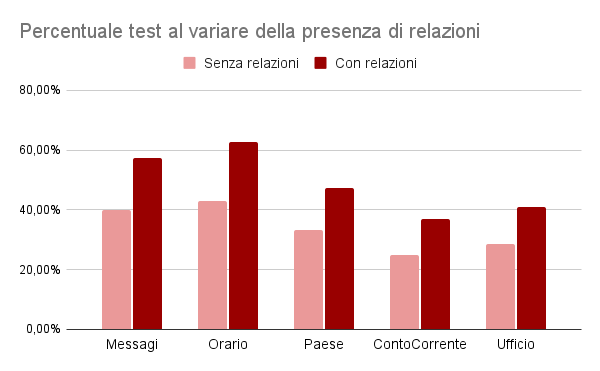
\includegraphics[width=14.5cm]{tesi refactoring/thesis/files/img/Percentuale test al variare della presenza di relazioni.png}
        \caption{Apporto valoriale delle relazioni tra classi nei test}
    \end{figure}
     Il grafico illustra la differenza tra i \textit{test} generati senza inserire nel \textit{prompt} le classi con relazioni a quella da testare e quelli 
    con l'aggiunta di classi inserite nel \textit{prompt}. È chiaramente visibile che la quantità di \textit{test} generati nel secondo caso è maggiore ma soprattutto il numero di \textit{test} che passano è notevolmente più alto.
    In particolare la generazione di \textit{test} includendo anche le classi in relazione ha generato mediamente il 15\% in più di \textit{test} corretti.
    Un quesito però che ricorre frequentemente nello sviluppo dei \gls{llm} è la \textit{large context window}, in particolare l'aggiunta dei \textit{related\_method} e delle \textit{related\_class} potrebbe portare ad alcuni problemi, tra cui la moltitudine di dati da processare e l'\textit{information overload}.
    In particolare l'\textit{information overload} potrebbe portare a un maggior \textit{focus} sugli \textit{edges} del \textit{context} se questo fosse troppo ampio, e ciò porterebbe a perdere il \textit{focus} sulle parti più importanti della domanda. È stato quindi importante affrontare questa sfida durante lo sviluppo per capire la quantità di metodi e classi relazionate alla classe della quali si voleva andare a generare \textit{test}.
    La seconda problematica riscontrata durante il parsing riguarda la tipizzazione dei linguaggi, in particolare l'analisi sintattica è stata senza dubbio un'attività dispendiosa in termini di tempo ed energia, poichè il linguaggio di programmazione Python, essendo non tipizzato, non presenta una distinzione chiara tra le istruzioni. In particolare, l'istanziazione di un oggetto è trattata come un'assegnazione, in mancanza di una parola chiave specifica. Pertanto, è plausibile ipotizzare che l'analisi sintattica in Java, un linguaggio tipizzato con restrizioni più rigorose, sia più agevole e conduca a risultati più accurati.
    % generazione script per scegliere classi da testare ed eseguire i test
    % generazione di filtri per migliorare i risultati e renderli adatti
    % scelgo progetto e classi, attraverso le relazioni tra classi e metodi, genero test
    % deduciamo che è importante trovare relazioni tra le classi, in linguaggi come Java è più semplice effettuare
    % parsing, in linguaggi privi di semantica invece è difficile andare a trovare queste relazioni e fare parsing.
    % è quindi anche più complesso effettuare il testing di queste classi poichè è difficile a monte trovare 
    % relazioni tra le classi e i metodi.
    
    \subsubsection{Generazione dei \textit{test}}
    Una volta completato il parsing del progetto, lo \textit{script} può essere avviato attraverso i comandi sopra citati.
    In particolare, il comando “python3 --genTestClass Class\_Name” permette di generare i \textit{test} per una particolare classe all'interno del nostro progetto.
    Quando si esegue questo comando, lo \textit{script} recupera la classe scelta all'interno del database e genera i test di unità per i metodi della classe stessa.
    Il secondo comando “python3 --genTestMethod Class\_Name Method\_Name” invece consente di generare i \textit{test} per un metodo specifico all'interno della classe.
    Come nel caso precedente, lo \textit{script} recupera la classe e il metodo scelti all'interno del database e genera i \textit{test} di unità per il metodo selezionato.
    La generazione dei \textit{test} può essere effettuata attraverso l'utilizzo della \textit{Hugging Face Inference API} o tramite un \textit{server} locale. 
    L'impiego di \textit{Hugging Face} consente l'utilizzo di modelli di dimensioni considerevoli, come ad esempio \textit{Llama3 70b}, i quali sono in grado di produrre test più accurati e corretti. Tuttavia, ciò comporta un rallentamento della velocità di inferenza e ad un aumento dei costi. 
    Dall'altro lato, l'utilizzo di un \textit{server} locale offre una maggiore velocità di inferenza, ma con l'impiego di modelli di dimensioni ridotte, come ad esempio \textit{Chat Qwen 1.5 1b q4}.
    % generazione di test attraverso llm 

    \subsection{\textit{Benchmarks}}
    % benchmarking degli LLM
    % generazione di test attraverso OpenAI e linguaggi invece addestrati su codice
    Dopo lo sviluppo dello \textit{script}, vi è stato un periodo di \textit{test} il quale è stato fondamentale principalmente per due scopi. 
    La prima motivazione è legata al miglioramento del \textit{prompt} per migliorare i risultati.
    Infatti, andando ad ottimizzare il prompt, in modo tale da poter produrre domande più specifiche e maggiormente comprensibili all'\gls{llm}  si possono ottentere \textit{test} più accurati 
    e corretti. 
    La seconda motivazione riguarda il confronto tra i vari \gls{llm} utilizzati.
    Volevo capire se l'utilizzo di \gls{llm} addestrati su codice sorgente fosse più efficace rispetto a quelli addestrati su testo generico, oltre a ciò volevo capire quale fosse l'\gls{llm} più adatto per il mio progetto.
    Ricordando che uno degli scopi principali del progetto è la ricerca dell’\gls{llm} più adeguato alle esigenze e alle possibilità di Zucchetti, 
    inizialmente ho proceduto alla ricerca della temperatura adeguata affinché il modello riuscisse a produrre risultati attendibili evitando 
    l’utilizzo di \gls{llm} molto pesanti. I dati ottenuti sono raffigurati nella figura 3.4 sottostante.\newpage
    \begin{figure}[!h]
        \centering        
        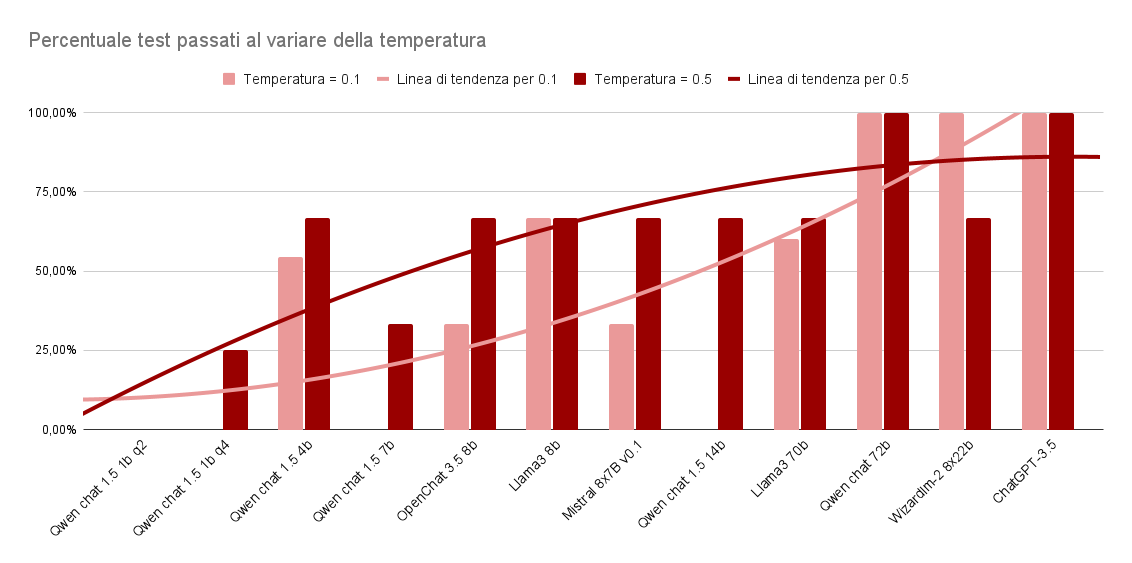
\includegraphics[width=14.5cm]{img/Percentuale test passati al variare della temperatura.png}
        \caption{Test generati attraverso temperature diverse}
    \end{figure}
    \\È noto che aumentando la temperatura, un \gls{llmg} produce dati meno deterministici e offre la possibilità di ottenere risultati più diversificati.
    Questo è particolarmente evidente nel caso di modelli con al massimo 14 miliardi di parametri. 
    In tal caso, diventa chiaro che mantenere un elevato grado di determinismo non comporta vantaggi significativi, 
    poiché il numero di parametri è minore e, di conseguenza, anche le conoscenze del modello sono limitate. Nel caso invece 
    di modelli più grandi questo vantaggio non si percepisce, ed anzi, in un caso in particolare la sua capacità di generazione di \textit{test} corretti diminuisce.
    Il secondo \textit{test} di rilievo riguarda l'impiego di codice commentato figura 3.5. Ho ipotizzato che fornendo maggiori dettagli all'\gls{llm}, 
    anche se in forma di linguaggio naturale, il modello potesse generare \textit{test} più efficaci. I risultati ottenuti sono indubbiamente 
    i più significativi, poiché l'aumento delle informazioni nei modelli più piccoli porta quasi sempre a risultati superiori rispetto 
    a quelli ottenuti con modelli più grandi. Inoltre, gli stessi modelli hanno prestazioni migliori su prompt con commenti rispetto a
     quelli privi di essi. Posso pertanto supporre che ciò sia dovuto al fatto che, avendo meno informazioni a disposizione, l'incremento di esse 
     attraverso il testo aggiuntivo possa notevolmente migliorare le capacità del modello.
    \begin{figure}[!h]
        \centering        
        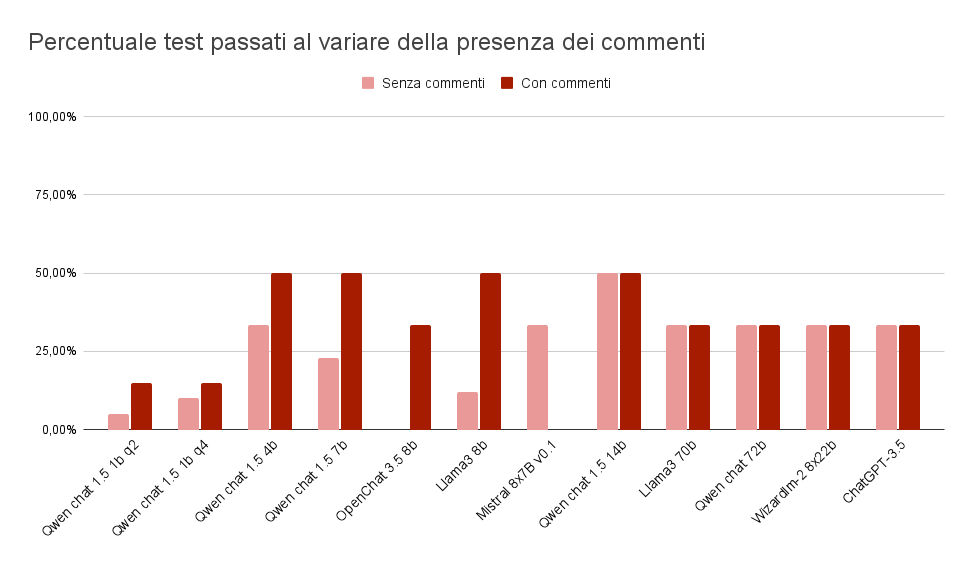
\includegraphics[width=14.5cm]{img/Percentuale test passati al variare della presenza dei commenti.png}
        \caption{Test generati attraverso temperature diverse}
    \end{figure}

 \newpage   Dopo queste rilevazioni, ho optato per confrontare la capacità di generazione di test su codice scritto in inglese e in italiano, questo perchè ho ipotizzato che
    la quantità di dati in italiano è minore rispetto a quella in inglese e quindi volevo capire se ci fossero differenze significative e se questa ipotesi fosse realmente vera.
    I risultati ottenuti sono raffigurati in figura 3.6 e figura 3.7.
    \begin{figure}[!h]
        \centering        
        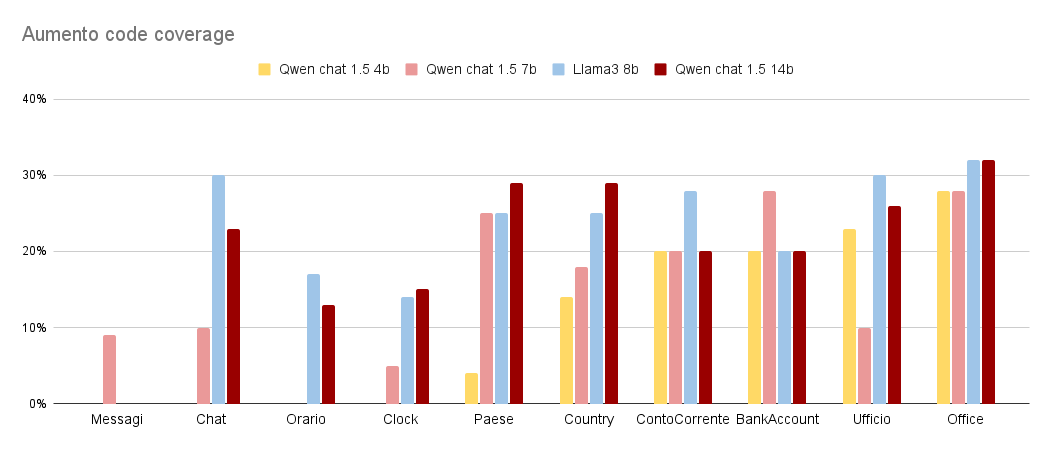
\includegraphics[width=14.5cm]{img/Aumento code coverage.png}
        \caption{Aumenti del code coverage al variare della lingua e dei modelli}
    \end{figure}
   \newline In figura 3.6  è sorprendente notare che in molti casi la quantità di \textit{code coverage} aumentata è molto simile tra \textit{llama 8b} e \textit{Qwen chat 14b}.
    In questi test quindi sebbene \textit{Qwen chat} sia addestrato su una mole di dati maggiore di \textit{llama}, i risultati sono molto simili.
    \begin{figure}[!h]
        \centering        
        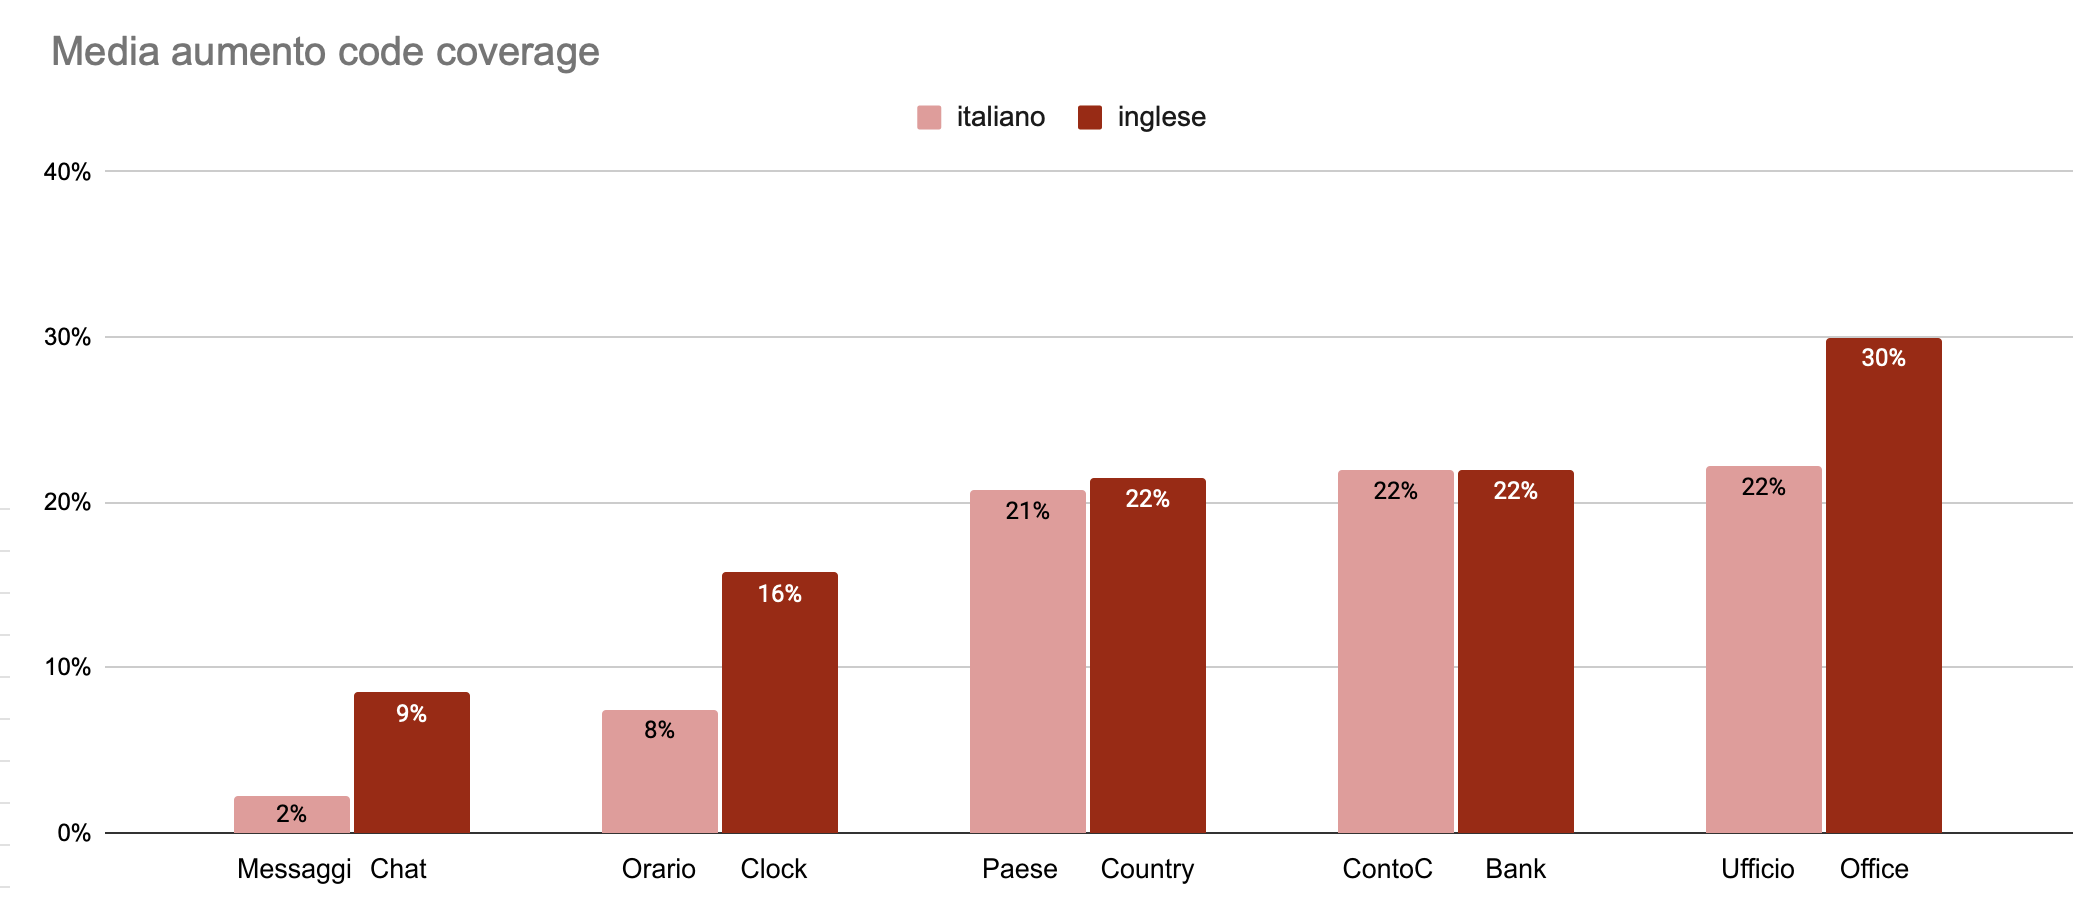
\includegraphics[width=14.5cm]{img/Media aumento code coverage.png}
        \caption{Media degli aumenti del code coverage al variare della lingua}
    \end{figure}
    \\In figura 3.7 notiamo invece che la media degli aumenti del \textit{code coverage} è sempre maggiore per le richieste su codice sorgente in inglese rispetto a quelle in italiano.
    L'ipotesi quindi che il codice in inglese possa ottenere risultati migliori rispetto a quello in italiano è confermata.
    \newpage
\section{Resoconto finale}
    In questa sezione si procederà a fornire un resoconto finale del lavoro svolto durante il primo macroperiodo, analizzando i risultati ottenuti e le problematiche affrontate.
    \subsection{Prodotti ottenuti}
    Durante il primo macroperiodo di lavoro sono stati ottenuti diversi risultati, tra cui la realizzazione di uno \textit{script} per l'estrazione e la generazione dei \textit{test} automatici.
    In particolare, lo \textit{script} permette di effettuare il parsing di un intero progetto, salvando i dati chiave all'interno di un database SQLite.
    Questo procedimento consente all'\gls{llm} di individuare le relazioni tra i vari metodi e le classi, facilitando la generazione dei \textit{test}.
    Inoltre, sono stati effettuati diversi \textit{benchmark} per valutare le prestazioni dei vari \gls{llm} utilizzati, confrontando i risultati ottenuti.

        %script python per generare test scegliendo le classi e analizzando i vari llm
        %lista prodotto ottenuto
    \subsection{Risultati ottenuti}
        I risultati ottenuti sono stati più che soddisfacenti, infatti, aver compreso l'importanza di avere un linguaggio tipizzato per l'analisi 
        sintattica è stato fondamentale per fornire risultati e costatazioni a Zucchetti.
        Inoltre, aver effettuato i \textit{benchmark} per valutare le prestazioni dei vari \gls{llm} utilizzati è stato un passo fondamentale 
        per capire quale fosse il modello e la tipologia di \textit{prompt} più adatto per un futuro sviluppo. 
        Nonostante il lavoro finora svolto risulti soddisfacente, persistono alcune aree di indagine e miglioramento. 
        Tra queste, si segnala la necessità di affrontare l'incertezza riguardante la correttezza del codice generato, 
        che può essere erroneo e deve essere scartato, oppure evidenziare la presenza di un difetto nel sistema, rendendolo di conseguenza un \textit{test} di rilevanza significativa.
        %\cite{article:Hu2021LoRALA}
        %problematiche relative al fatto che se non applico filtri di LLMSE il modello non è in grado di generare codice sorgente valido
        %ma non so se questo codice non è valido perchè è errato o perchè ha trovato un bug
    \subsection{Conclusione}
        %conclusione di tutto il lavoro svolto quindi prodotto         
        % bene o male, pro e contro del PROGETTO e di come è stato affrontato
        Durante l'implementazione del progetto, mi sono imbattuto in diverse sfide, tra cui la complessità dell'analisi sintattica in linguaggi non tipizzati, 
        come nel caso di Python e la complessità del funzionamento delle reti neurali. Una difficoltà aggiuntiva è stata rappresentata dalla limitatezza delle risorse computazionali disponibili. 
        Pur facendo stage un'azienda di rilievo come Zucchetti, le risorse a disposizione non sono state sufficienti per l'utilizzo frequente di modelli linguistici di grandi dimensioni, 
        come Mixtral 7x8b o Wizardlm-2 8x22b. Inoltre, la natura intricata del progetto e la scarsità di materiale informativo relativo all'argomento \gls{llmse} hanno costituito ulteriori ostacoli. 
        È importante notare che \gls{llmseg} è ancora un argomento in fase embrionale, il che si traduce in una carenza di risorse documentative a riguardo. Nonostante queste sfide, 
        il primo macroperiodo del progetto è stato affrontato con successo, generando risultati significativi e fornendo basi solide per uno sviluppo futuro.
\newpage
     \chapter{Fine-tuning di LLM attraverso LoRA e ottimizzazioni}
\label{chap:descrizione-stage-2}
\section{Analisi del dominio applicativo}
Nella seconda fase del progetto si è proceduto con il \gls{fine-tuning} di un \gls{llm} attraverso \gls{lora}, e le sue ottimizzazioni, come ad esempio \textit{MoLE} e \textit{AdaMoLE}. In questo capitolo si approfondiranno inoltre gli studi effettuati sul \gls{fine-tuning} e quantizzazione, concentrandosi maggiormente sul possibile apporto valoriale che questi ultimi possono dare ad un \gls{llm} e alle sue implementazioni.
Questo poichè moltissime realtà aziendali si stanno concentrando sul \gls{fine-tuning} di modelli preaddestrati, in quanto permette di adattare un modello ad un nuovo dominio, senza doverlo addestrare da zero.
%porzione del mondo reale con cui si deve interagire
    \subsection{Analisi del tema}
    Nella seconda parte del progetto, vi è stata una maggiore attenzione posta principalmente sullo studio delle tecniche di \gls{fine-tuning} e quantizzazione, poiché rappresentano argomenti complessi e nuovi nel settore. In particolare, la lettura di diversi articoli scientifici e la realizzazione di esperimenti su \textit{Colab} sono stati fondamentali per comprendere a fondo queste tecniche. Queste attività sono state inoltre indispensabili per poter applicare in modo pratico le nozioni apprese.
    Questa fase del progetto si distingue inoltre dalla prima poiché si è focalizzata maggiormente sulla ricerca e sperimentazione di nuove metodologie rispetto all'applicazione pratica immediata. Tuttavia, sebbene il focus principale fosse la ricerca, vi è stata comunque la possibilità di applicare queste tecniche in modo pratico tramite l'utilizzo di \textit{Colab}.

    %descrive il dominio del problema da affrontare:
    %la porzione del mondo reale, rilevante per il sistema\\
    %-> Su cui si devono mantenere informazioni\\
    %-> Concuisideve interagire

    %LoRA e quantizzazione -> perchè sono utilizzati 

    \subsection{Esempi di utilizzo}
   Al giorno d'oggi, le possibili applicazioni di un \gls{llm} \textit{fine-tuned} sono molteplici e spaziano dalla generazione di codice sorgente alla traduzione di testi. Queste tipologie di utilizzo sono chiamate \textit{downstream task}, poiché sono \textit{task} eseguite dopo il preaddestramento del modello e si concentrano su argomenti specifici. Le \textit{downstream task} rappresentano quindi la motivazione principale per effettuare il \gls{fine-tuning} di un modello preaddestrato. Lo scopo di questa attività è far concentrare il modello su un particolare dominio, migliorando così le performance in quei compiti specifici rispetto a un modello preaddestrato generico.
Per quanto riguarda la quantizzazione, l'utilizzo di modelli quantizzati è oggi pressoché fondamentale. I modelli non quantizzati richiedono infatti troppa memoria e potenza di calcolo, rendendo difficile per la maggior parte delle aziende utilizzare modelli di \gls{llm} senza questa tecnica di ottimizzazione.

    %dare la possibilità all'LLM di rispondere a domande sul dominio downstram task
    % rendere disponible i modelli anche su macchine più piccole ad esempio microcontrollori
    \subsection{LoRA}
    \gls{lora} è un metodo di \gls{peft} che permette di adattare un modello preaddestrato ad un nuovo dominio, attraverso l'aggiunta di un \textit{layer}.
    Questa metodologia di \gls{fine-tuning} viene introdotta da J. Edward Hu et al.\cite{article:Hu2021LoRALA} e consiste nel congelare i pesi del modello preaddestrato e inserire delle \textit{trainable rank decomposition matrices} come un \textit{layer} aggiuntivo.
    Queste matrici permettono di diminuire notevolmente il numero di parametri da addestrare, rendendo il \gls{fine-tuning} più veloce e meno costoso.
    La costruzione delle \textit{trainable rank decomposition matrices} A e B avviene attraverso la decomposizione di della matrice di pesi W in due matrici di rango ridotto.
    Supponiamo di avere una matrice preaddestrata $W_0 \in \mathbb{R}^d^\times^k$, e voler aggiungere un \textit{layer} $\Delta W$ per il fine tuning, allora possiamo scrivere:\newline 
    \centerline{$ W_0 + \Delta W = W_0 + BA$ ,}
    \newline 
    dove $B \in \mathbb{R}^d^\times^r$ e $A \in \mathbb{R}^r^\times^k$ con rank $r \ll min(d, k)$. 
    In questo modo è possibile addestrare solamente un insieme più piccolo di parametri i quali, moltiplicati tra loro, si avvicinano alla matrice di pesi più ampia nel modello pre-addestrato.
    \begin{figure}[htp]
        \centering
        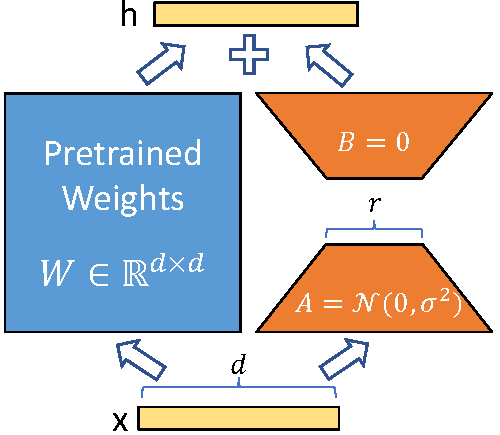
\includegraphics[alt={Testo alternativo dell'immagine}, width=0.5\columnwidth]{img/figure1.pdf}
        \caption{LoRA matrices}
        \label{fig:entanglement}
    \end{figure}
    \newline
    $A$ e $B$ vengono rispettivamente inizializzati attraverso la funzione Gaussiana e 0, quindi il valore all'inizio dell'addestramento della matrice $W$ è 0. Attraverso le iterazioni, i parametri verranno modificati e si otterrà un \textit{layer} LoRA che permetterà al modello di avere capacità più specifiche.
    Notiamo quindi che la quantità di dati da aggiornare è nettamente minore, si dovrà infatti addestrare solo $A$ e $B$. In particolare, l'utilizzo della VRAM diminuisce di 2/3 se  $r \ll d_m_o_d_e_l$.
    L'utilizzo di \gls{lora} porta ad alcuni vantaggi oltre al risparmio di memoria, l'addestramento infatti risulta più efficiente ed inoltre è possibile creare tanti \textit{layers} \gls{lora} in modo da poterli interscambiare in base alle esigenze.
    %cos'è, come funziona e spiegazione matematica con qualche immagine delle matrici
    \subsubsection{Future applicazioni} 
    Le future applicazioni che durante questo stage sono state prese in considerazione con il tutor aziendale Gregorio Piccoli e sono legate soprattutto alla possibilità di utilizzare modelli 
    \textit{fine-tuned} per rispondere a domande sul dominio \textit{downstream task}, come ad esempio la generazione di codice sorgente.
    Un ulteriore utilizzo potrebbe essere legato al compilatore dei linguaggi di programmazione, in modo tale da avere un feedback logico del programma oltre che sintattico e semantico.
    Inoltre, un'altra possibile applicazione è quella di rendere disponibili i modelli attraverso la quantizzazione anche su macchine più piccole, come ad esempio microcontrollori. Questa possibilità al giorno d'oggi permetterebbe l'utilizzo 
    di \gls{llm} in dispositivi che non hanno una potenza di calcolo elevata, come ad esempio gli smartphone.

    
\section{Analisi dei requisiti}
    \subsection{Analisi preventiva dei rischi}
    Durante la fase di analisi dei rischi sono stati individuate le possibili criticità che potranno essere riscontrate.
    Si è quindi proceduto a elaborare delle possibili soluzioni per far fronte a tali rischi.
    \begin{risk}{Mancanza di risorse computazionali}
        \riskdescription{Essendo il \gls{fine-tuning} un processo molto oneroso, la quantità di risorse computazionali a disposizione potrebbe risultare quindi non sufficiente per addestrare modelli molto grandi}
        \risksolution{utilizzo di Colab e coinvolgimento del responabile aziendale}
        \label{risk:data-absence} 
    \end{risk}

    \subsection{Requisiti e obiettivi}

    \begin{center}
        \rowcolors{1}{}{tableGray}
        \begin{longtable}{|p{2.25cm}|p{7.75cm}|p{2.25cm}|}
        \hline
        \multicolumn{1}{|c|}{\textbf{Obiettivo}} & \multicolumn{1}{c|}{\textbf{Descrizione}}\\ 
        \hline 
        \endfirsthead
        \multicolumn{3}{c}%
        {{\bfseries \tablename\ \thetable{} -- Continuo della tabella}}\\
        \hline
        \multicolumn{1}{|c|}{\textbf{Obiettivo}} & \multicolumn{1}{c|}{Descrizione}\\ \hline 
        \endhead
        \hline
        \multicolumn{3}{|r|}{{Continua nella prossima pagina...}}\\
        \hline
        \endfoot
        \endlastfoot 
        OB 4 & Realizzazione di test con LLM fine-tuned attraverso \gls{lora}. \\
        \hline
        DE 1 & Quantizzazione di LLM. \\
        \hiderowcolors
        \caption{Requisiti secondo macroperiodo.}
        \label{tab:requisiti_obbiettivi}
        \end{longtable}
    \end{center}



\section{Sviluppo del prodotto}
Lo sviluppo del prodotto durante il secondo macroperiodo non è stato immediato come è successo durante prima  parte, questo poichè è stato necessario studiare in modo approfondito gli argomenti che sarebbero stati trattati successivamente. Dopo lo studio della teorica legata al \gls{fine-tuning} e  quantizzazione, è stato necessario studiare anche le tecniche di applicazione, ciò è avvenuto simultanemanete alla loro implementazione, vi è stato quindi un'applicazione della metodologia di apprendimento \textit{learing by doing}.
Inoltre, è stato necessario preparare un dataset attraverso il quale effettuare il \gls{fine-tuning}.
%studio iniziale di LoRA e quantizzazione perchè sono argomenti complessi e nuovi
%trovare dataset con il quale fare fine-tuning
    \subsection{\textit{Fine-tuning attraverso Pytorch}}
     Il \gls{fine-tuning} è un processo costoso, per questo motivo si è scelto di eseguirlo su \textit{Colab}, utilizzando un account Pro, il quale offre 100 unità di calcolo. Di seguito viene spiegato il processo di \gls{fine-tuning} attraverso il codice utilizzato.
     È possibile in figura 4.2 trovare il codice relativo alla configurazione di \gls{lora}.
    %CODICE LoRA
    \begin{figure}[!h]
        \centering        
        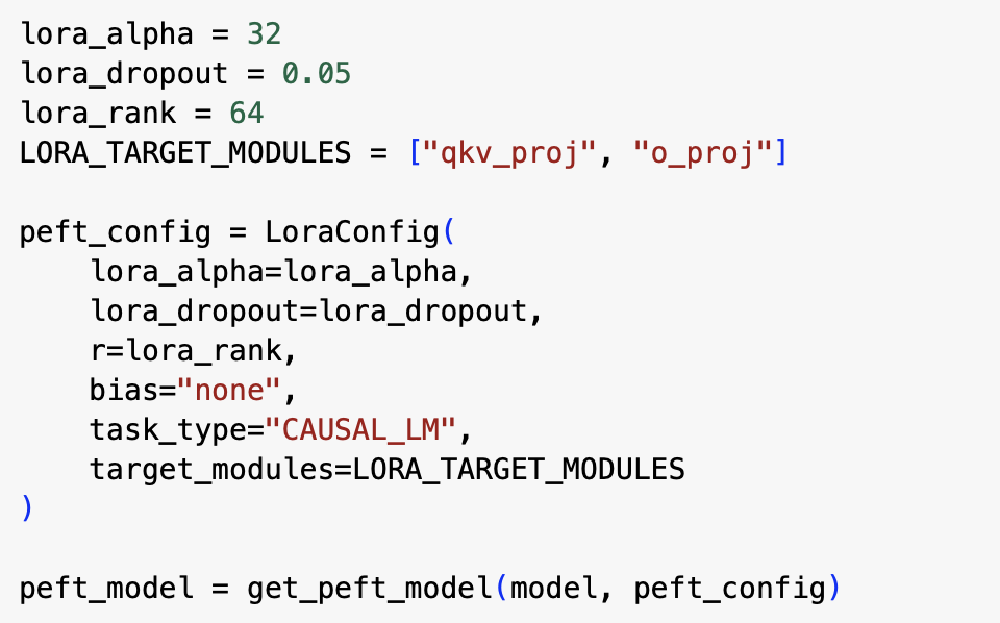
\includegraphics[width=12cm]{img/codiceLoRA.pdf}
        \caption{Configurazione parametri \gls{lora}}
    \end{figure}\newline
\begin{itemize}
    \item \textbf{lora\_alpha} determina l'entità della riduzione del rango durante il processo di approssimazione \textit{Low Rank}. Un valore più alto di \textit{lora\_alpha} comporta una riduzione più aggressiva del rango, risultando in una maggiore compressione delle matrici dei pesi e in un modello più efficiente in termini di parametri. Al contrario, un valore inferiore di \textit{lora\_alpha} comporta una riduzione meno aggressiva del rango, preservando più parametri del modello originale.
    \item \textbf{lora\_rank} esprime invece il rango della matrice decomposta. Un rango maggiore implica un maggiore utilizzo di memoria, mentre un rango minore riduce l'impatto sulla memoria ma comporta una perdita di informazioni. Diventa quindi cruciale trovare il rango più adeguato per bilanciare l'efficienza della memoria e la conservazione delle informazioni.
    \item \textbf{lora\_dropout} è la probabilità di eliminare elementi dalle matrici $A $ e $B$ per evitare \textit{overfitting}.
    \item \textbf{LORA\_TARGET\_MODULES} sono i moduli dei layer ai quali verrà applicato \gls{lora}. In questo caso, \gls{lora} è stato applicato ai moduli \textit{qkv\_proj}, \textit{o\_proj} presenti come visibile in figura 4.4 nella \textit{self attention} come suggerito da et al. \cite{article:Hu2021LoRALA} .
    È importante notare che i moduli in questione potrebbero cambiare in base al modello e alla sua architettura interna.
    \end{itemize}

In figura 4.3 è possibile quindi visualizzare l'architettura di \textit{Phi3-mini}, uno dei modelli al quale è stato applicato il \gls{fine-tuning}, \textit{Phi3-mini} è un \textit{state-of-the-art open model} , il quale si basa sull'architettura \textit{Transformer} ed è stato pre-addestrato sia con dati pubblici ma anche sintetici. 
    \begin{figure}[!h]
        \centering        
        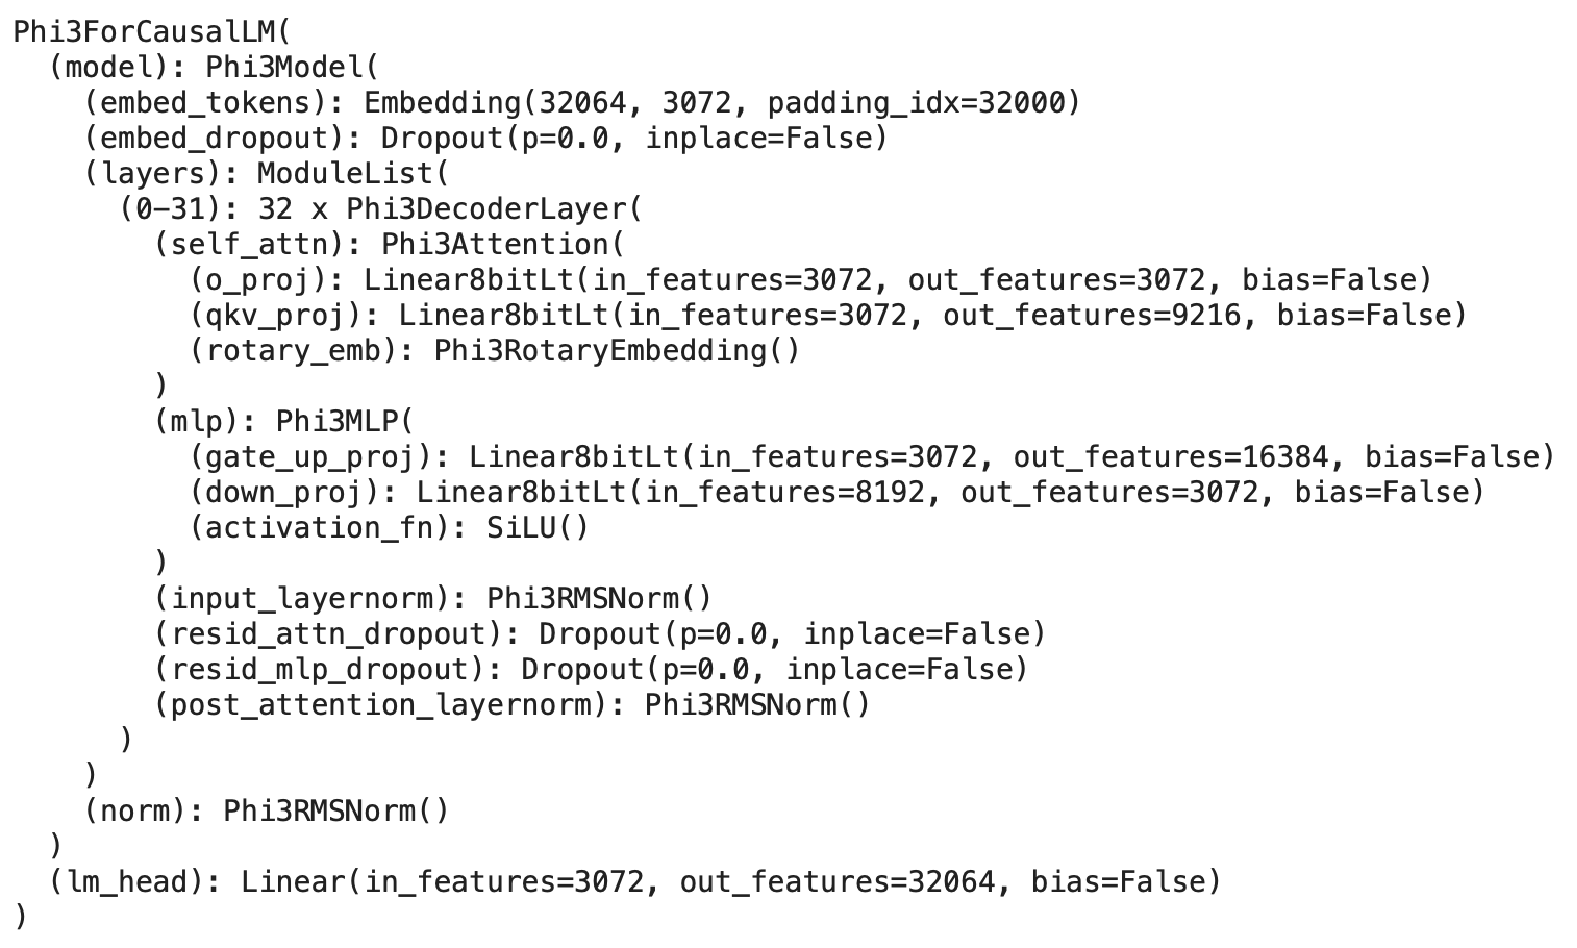
\includegraphics[width=14.5cm]{img/Phi3.pdf}
        \caption{Architettura di \textit{Phi3-mini}}
    \end{figure}

    \begin{figure}[!h]
        \centering        
        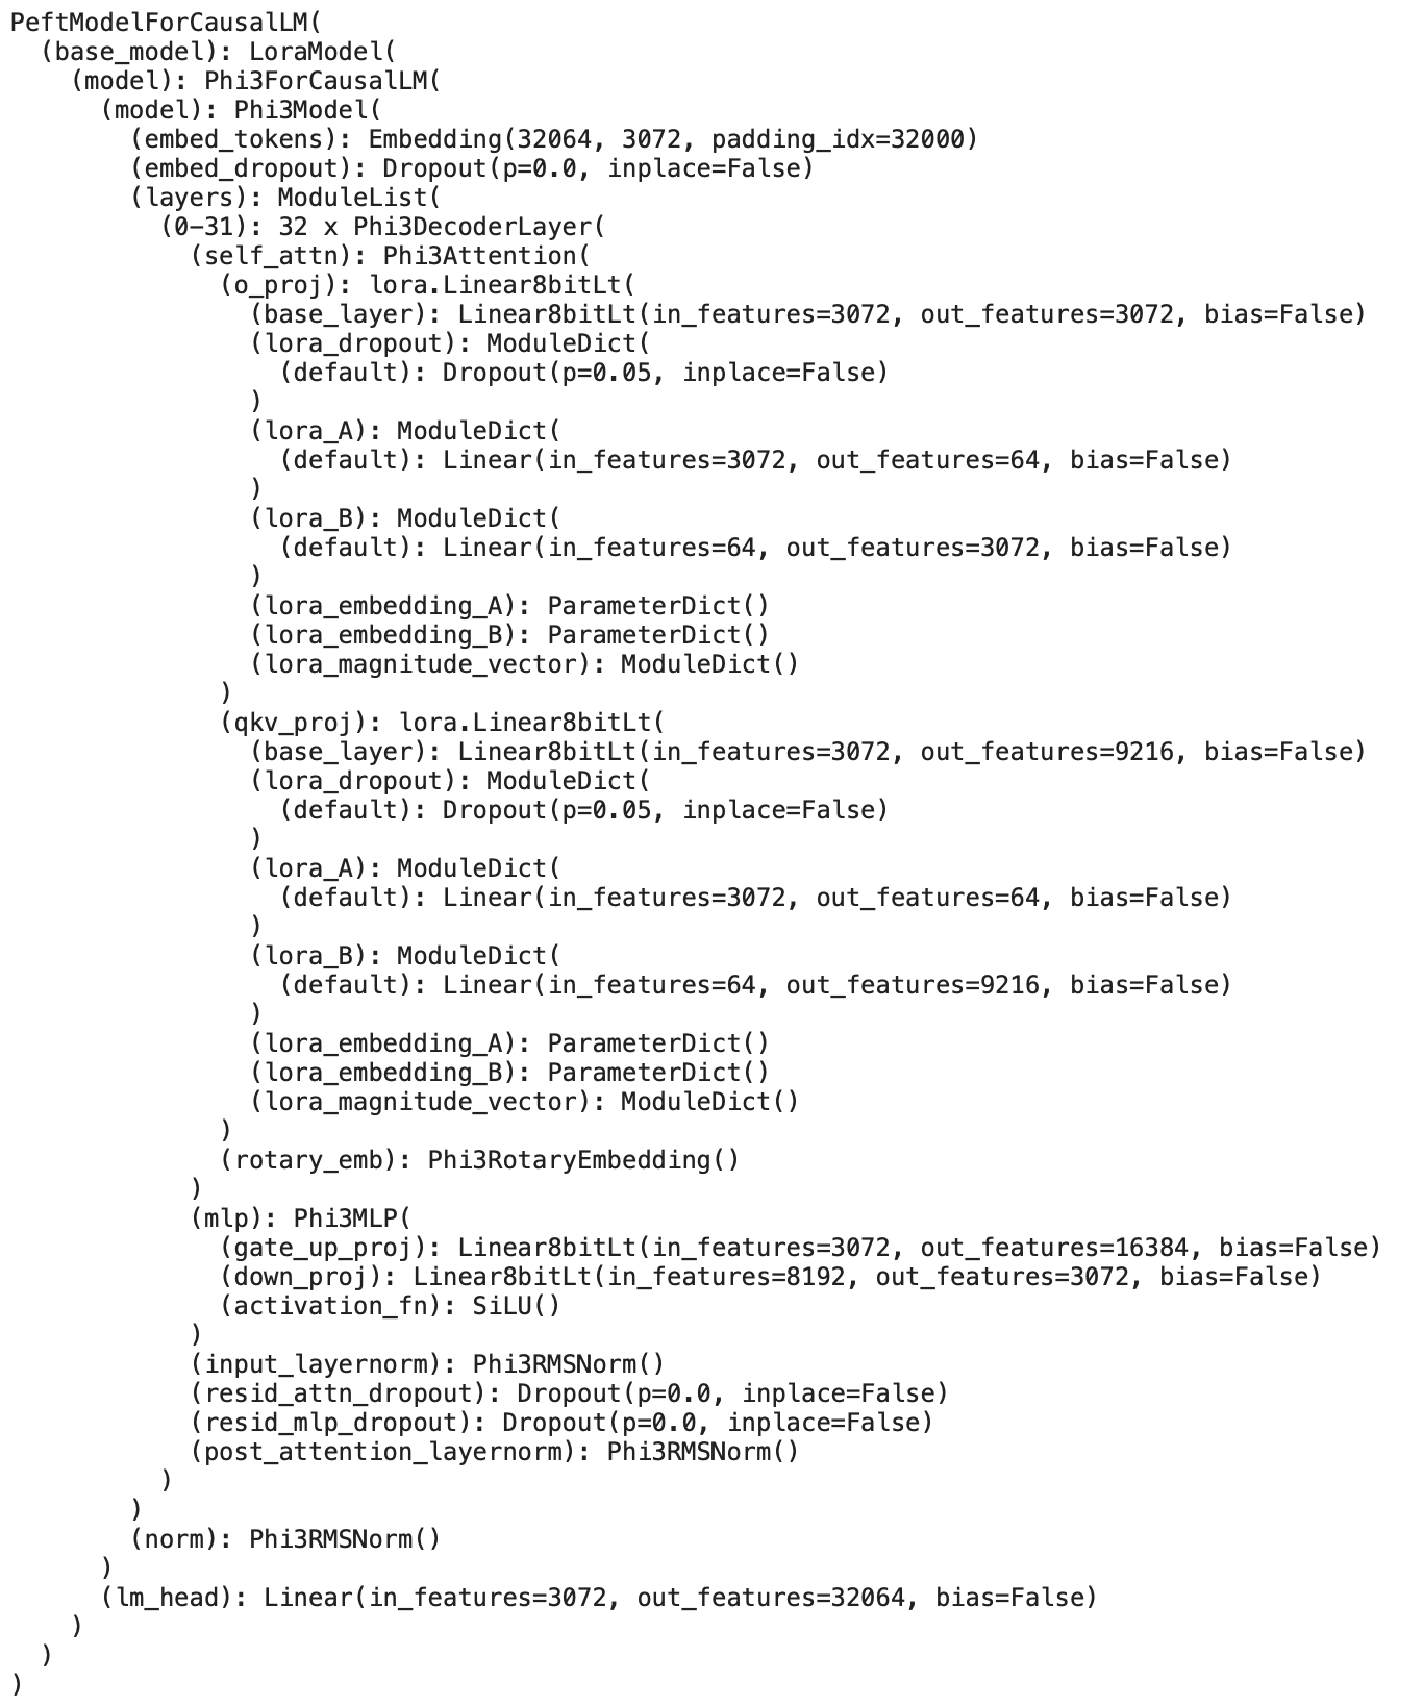
\includegraphics[width=14.5cm]{img/LoRA.pdf}
        \caption{Applicazione \gls{lora} a \textit{Phi3-mini}}
    \end{figure}\newpage
    
    Nella figura 4.4 possiamo notare il risultato ottenuto dall'applicazione di \gls{lora}. 
    
    %scrivi che si vede che lora è applicato ed infatti si vede che ci sono i layer sui moduli e sono di grandezza 64
    
    Successivamente, è stato necessario trovare un \textit{dataset} appropriato per il \gls{fine-tuning}. È stato scelto "\textit{Vezora/Tested-22k-Python-Alpaca}", che contiene ben 22.600 esempi di codice testato. Il dataset, suddiviso in istruzioni, input e output, è stato formattato correttamente come mostrato in figura 4.5 per seguire il \textit{prompt} con cui il modello di partenza è stato addestrato. Questo passaggio è cruciale poiché ogni \gls{llm} richiede un determinato \textit{prompt}. Senza il \textit{prompt} adeguato, il modello non riuscirebbe a riconoscere i delimitatori utilizzati per distinguere le istruzioni dalle corrispondenti risposte.

    \begin{figure}[htp]
        \centering        
        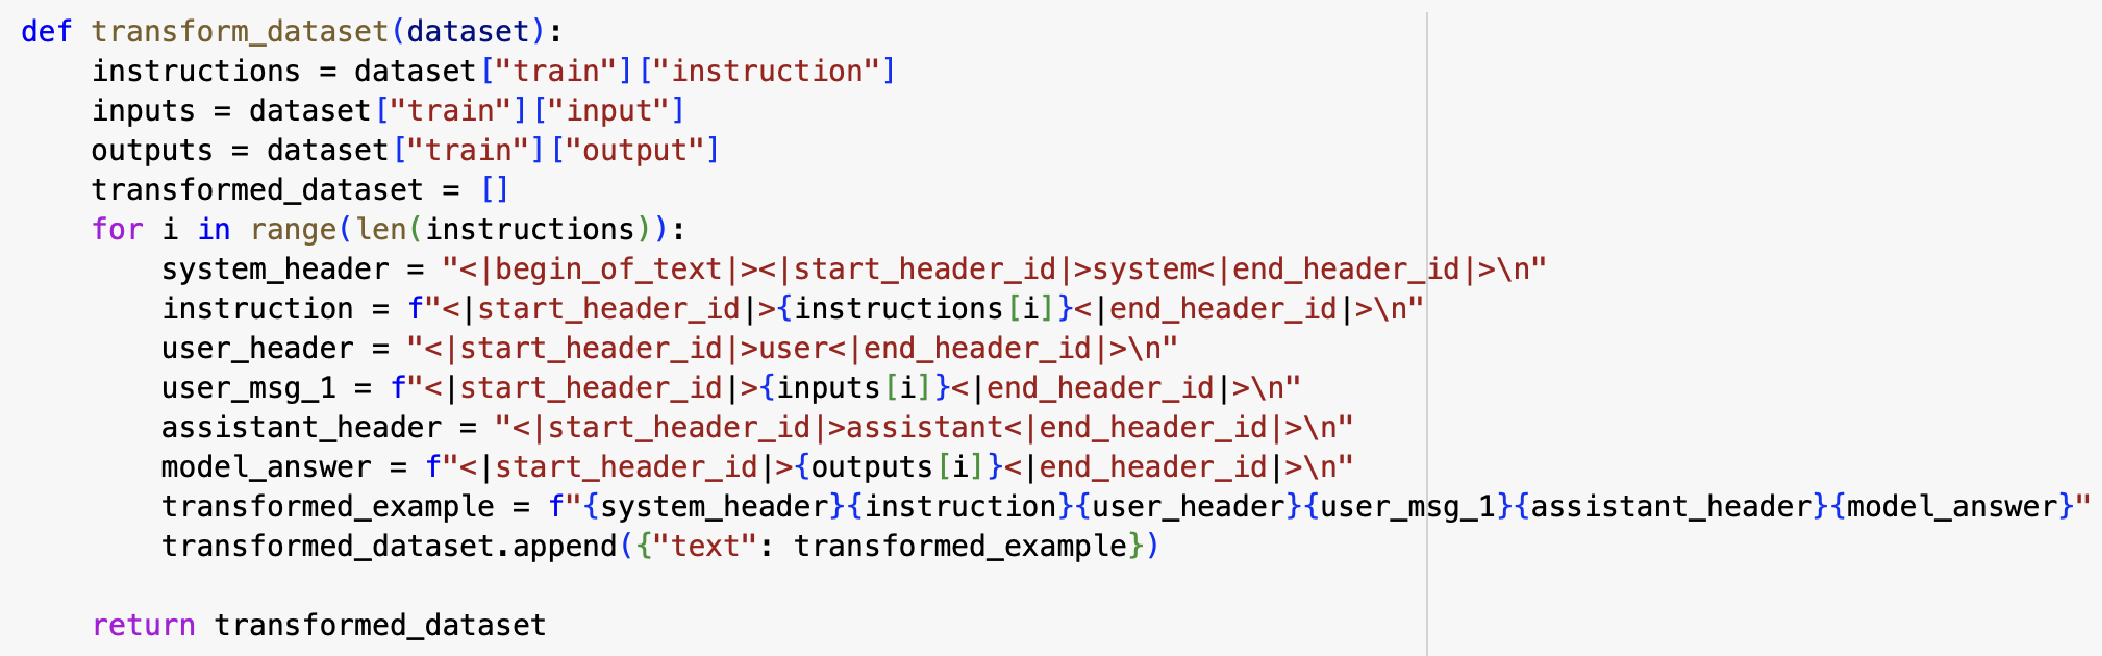
\includegraphics[width=14.5cm]{img/promptFormat.pdf}
        \caption{Funzione per costruire il \textit{prompt} adeguato a \textit{Phi3-mini}}
    \end{figure}\newline
    %PROMPT FORMAT CODICE
    %perchè il prompt è importante
    L'ultimo passaggio prima di effetturare effettivamente il \gls{fine-tuning} è stato definire i parametri per l'allenamento, come ad esempio \textit{per\_device\_batch\_size}, \textit{optim}, \textit{learning\_rate}, \textit{max\_step}.
    In questo caso si è deciso di avere una grandezza di \textit{batch} pari a 16, ciò va a specificare il numero di esempi utilizzati per ogni iterazione del \textit{fine-tuning} del modello. 
    Rigurardo a \textit{optim}, l'ottimizzatore, si è deciso di utilizzare \textit{adamw\_torch} il quale è un algorimo di ottimizzazione che unisce i benefit dell'ottimizzatore \textit{Adam} con \textit{weight decay} (regolarizzazione) per prevenire l'\textit{overfitting}.
    La \textit{learning\_rate} invece è il tasso di apprendimento e determina quanto velocemente o lentamente un modello apprende. È un fattore di scalatura che regola quanto devono essere aggiornati i pesi del modello in risposta all'errore calcolato in ogni iterazione dell'addestramento. Per questo parametro è stato scelto $5\times10^-^5$ poichè dopo alcuni esperimenti è risultato essere il miglior valore di \textit{tradeoff} tra velocità e precisione.
    \begin{figure}[htp]
        \centering        
        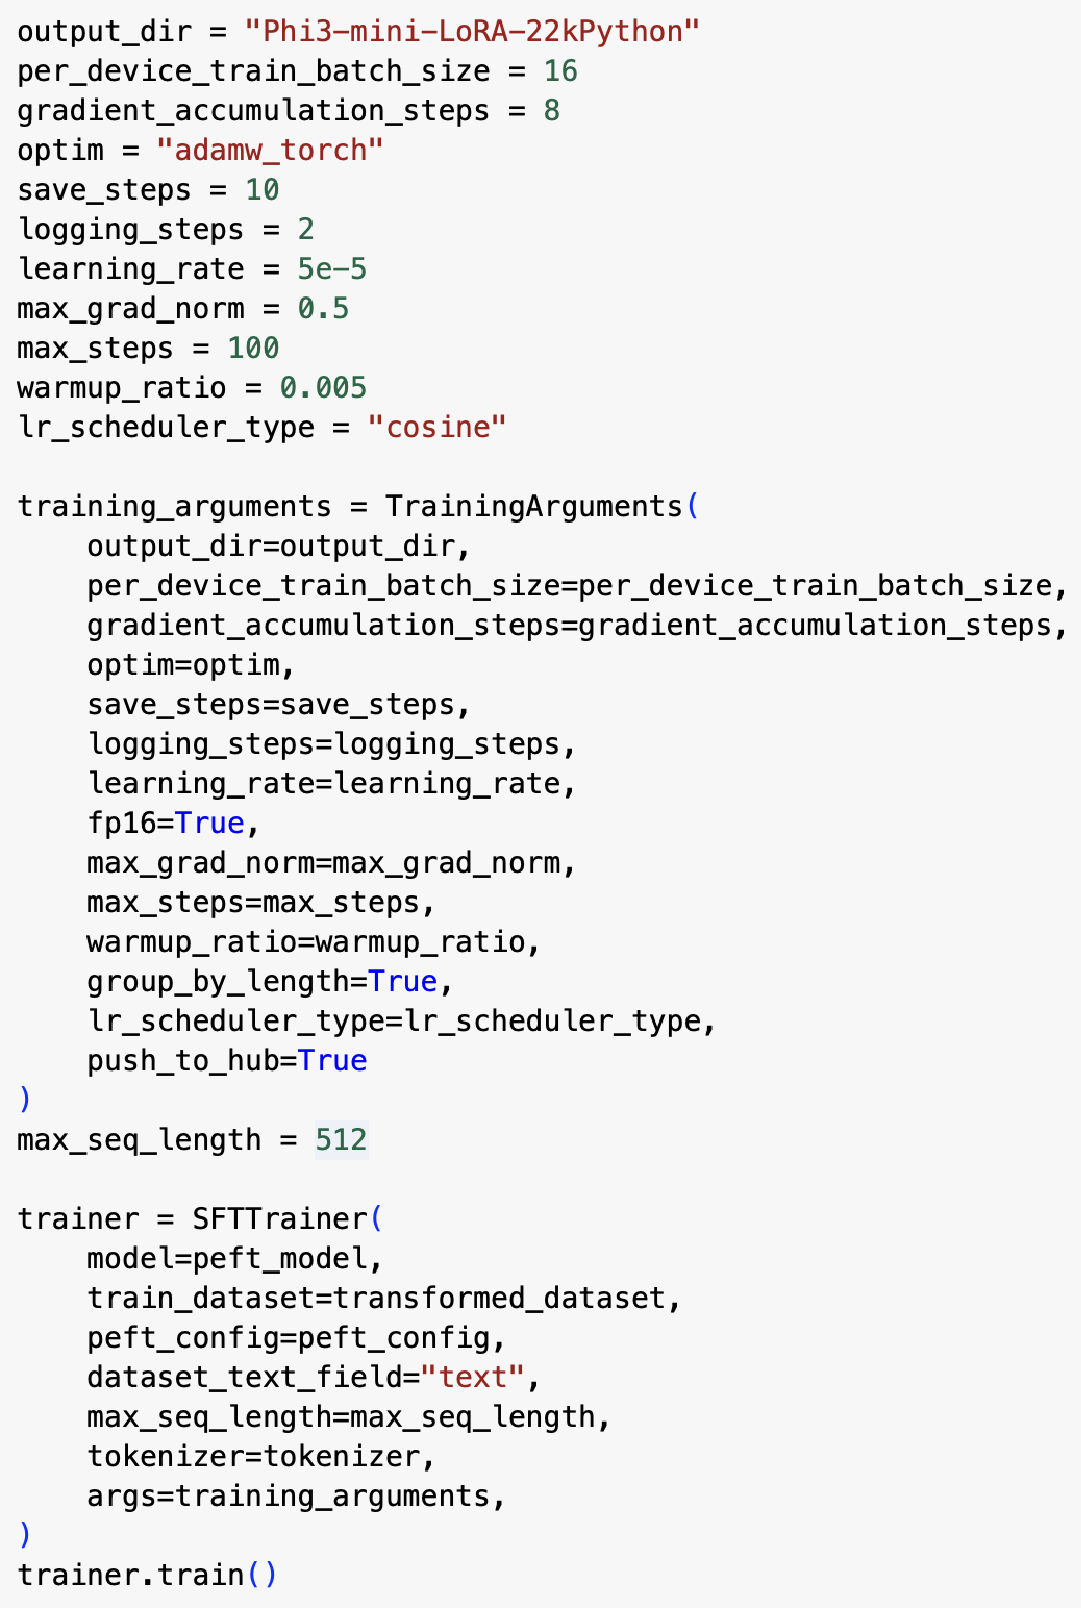
\includegraphics[width=12cm]{img/training.pdf}
        \caption{Esempio di codice per l'addestramento}
    \end{figure}\newpage

    %spiega il training


    \subsection{\textit{Fine-tuning attraverso LLama.cpp}}
      Oltre all'utilizzo di \textit{Colab}, è stato successivamente eseguito il \gls{fine-tuning} attraverso \textit{LLama.cpp}. A differenza di \textit{Colab}, \textit{LLama.cpp} prevede una semplificazione del codice e consente di utilizzarlo senza limiti computazionali, salvo quelli imposti dalle proprie risorse hardware.
    \begin{lstlisting}[language=bash]
        llama.cpp\finetune.exe
            --model-base model.gguf
            --train-data trainer.txt
            --lora-out Lora.gguf
            --threads 14
            --batch 8
            --sample-start "<s>"
            --ctx 1024
            --use-checkpointing
            --checkpoint-out LoRAModelCheckpoint-ITERATION.gguf
            --adam-iter 8192
            --adam-alpha 0.001
            --lora-r 16
            --lora-alpha 16
            --fill-with-next-samples
            --epoch 3
            --separate-with-eos
    \end{lstlisting}
    
    %fine tuning con LLamacpp -> comando e quanto ci ha messo 
        \subsection{Ottimizzazioni del fine-tuning}
        \subsubsection{Mixture of LoRA Experts}
        % estrai info da paper
        Il framework \textit{Mixture of} \gls{lora} \textit{Expert} rappresenta un metodo di \gls{fine-tuning} che si basa sull'utilizzo di \gls{lora}. Introdotta per la prima volta da Wu et al. \cite{article:Wu2024MixtureOL}, questa tecnica mira a risolvere i problemi legati alla riduzione delle capacità generative dei modelli affinati tramite \gls{lora}.
        Nel contesto di un modello \textit{Mixture of} \gls{lora} \textit{Expert} nell'apprendimento automatico, una funzione di gating viene utilizzata per assegnare dinamicamente diversi input a diversi "esperti" (tipicamente sub-modelli o reti neurali) all'interno del modello complessivo come visibile in figura 4.7. La funzione di gating:\\
        \centerline{$ \sigma(W\times x + b)$,} determina il contributo o il peso di ciascun esperto per un dato input, decidendo efficacemente quale esperto o combinazione di esperti debba essere responsabile delle predizioni per quell'input.\\
        \begin{figure}[htp]
            \centering        
            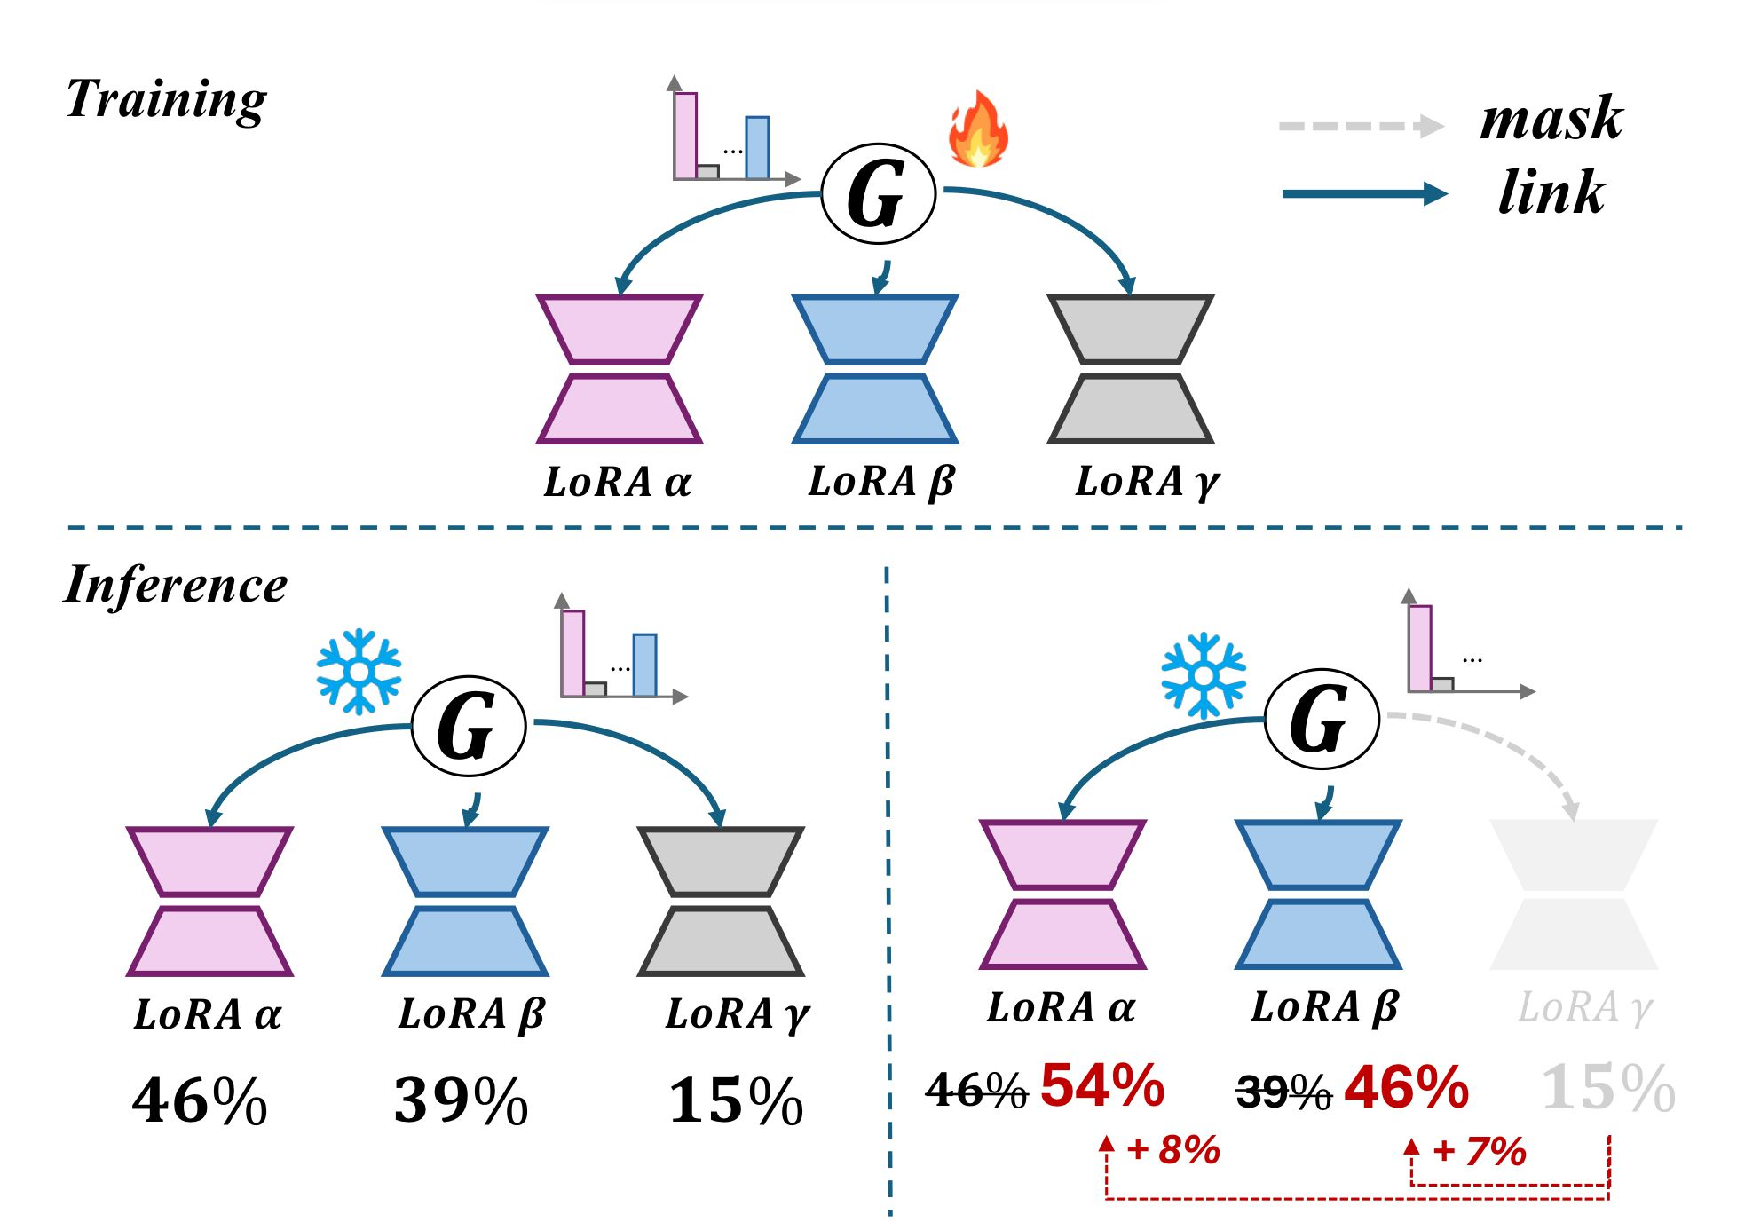
\includegraphics[width=10cm]{img/MoE2.pdf}
            \caption{Assegnazione dinamica dei LoRA \textit{layer} in Mixture of LoRA Expert}
        \end{figure}
       \newpage\textit{Mixture of} \gls{lora} \textit{Expert} consente l'impiego di diversi livelli di \gls{lora}, trattando ciascun livello addestrato con \gls{lora} come un esperto distinto. Implementa inoltre un controllo gerarchico del peso attraverso una funzione di gating che viene appresa all'interno di ogni livello, mantenendo congelati tutti gli altri parametri. In questo modo, è possibile apprendere pesi di composizione adattati specificamente agli obiettivi di un determinato dominio.
        \begin{figure}[htp]
            \centering        
            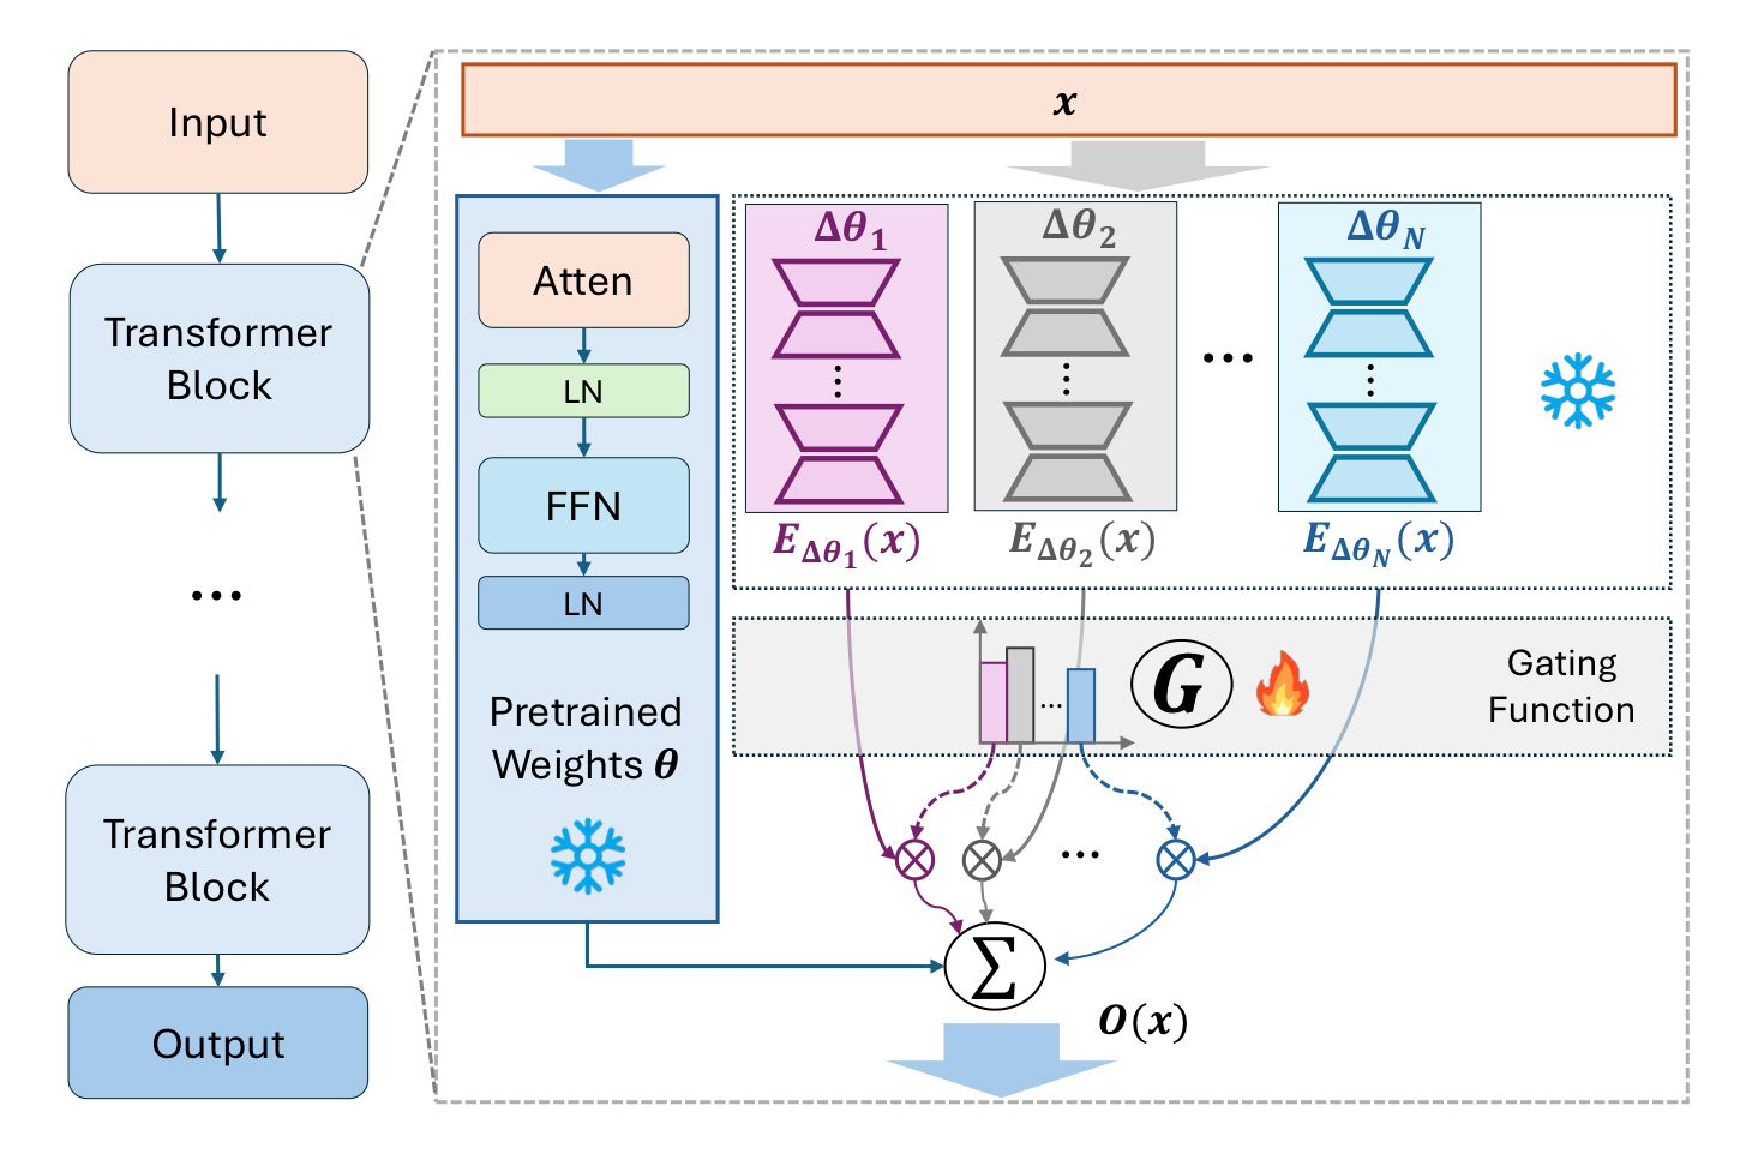
\includegraphics[width=10cm]{img/MoE1.pdf}
            \caption{Mixture of Expert all'intenro dell'architettura Transformer}
        \end{figure}

        
        I \textit{layer} quindi vengono integrati all'interno dell'architettura Transformer come visibile in figura 4.8.
        Come è visibile, l'idea di base di \gls{lora}, la quale consiste nel congelare i pesi pre-addestrati, continua ad essere presente, in parallelo, i \gls{lora} \textit{layer} dopo essere stati addestrati per specifiche \textit{task}, vengono sommati linearmente e il loro peso in questa somma viene determinato dalla funzione di gating.


        % MoLE -> 
        \subsubsection{AdaMoLE}
        \textit{Adaptive Mixture of} \gls{lora} \textit{Expert} è un metodo il quale utilizza \textit{Mixture of} \gls{lora} \textit{Expert} e una soglia di rilevanza, quest’ultima permette l’attivazione dei vari esperti solo se la loro percentuale di congruenza rispetto al contesto supera la soglia stessa.
        Questo procedimento permette una selezione dinamica degli   esperti attivando quindi solamente gli esperti che sono più appropriati rispetto al contesto (\textit{context-responsive}), ciò porta ad una migliore adattabilità e performance più elevate.
        \begin{figure}[htp]
            \centering        
            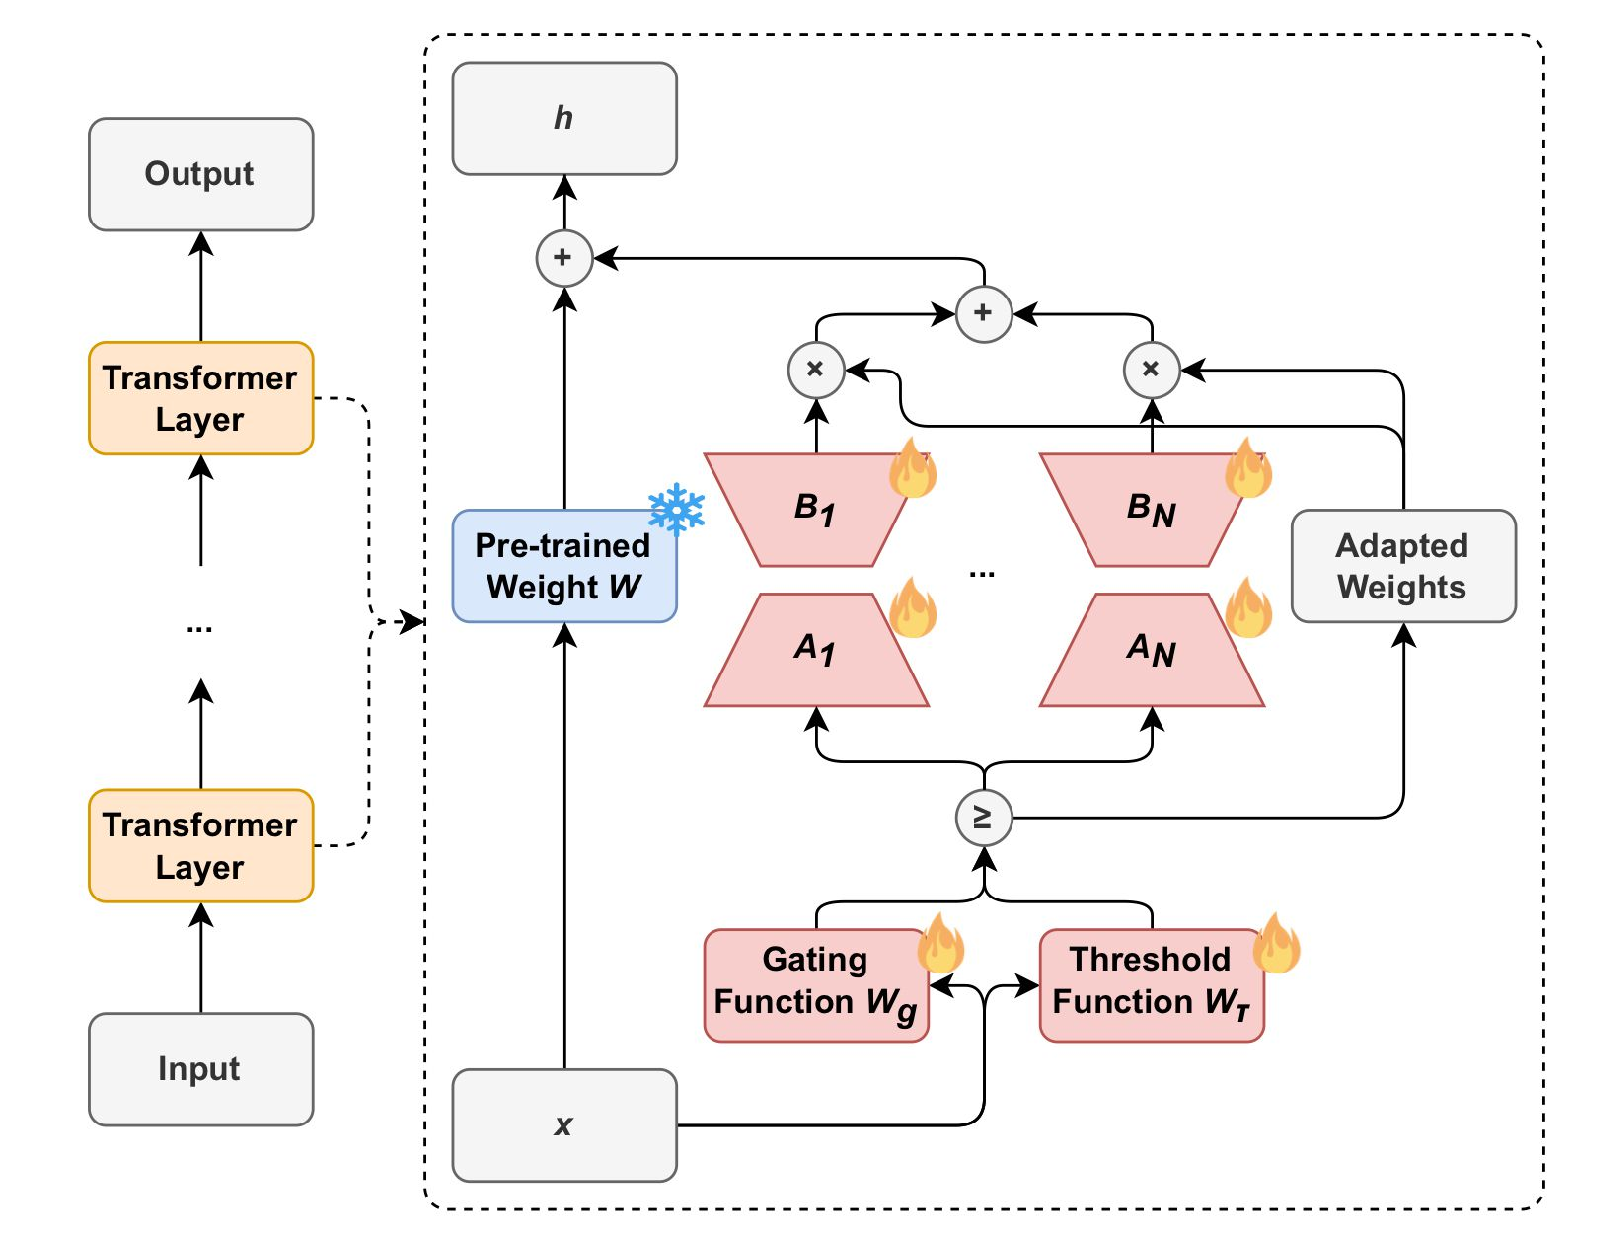
\includegraphics[width=10cm]{img/AdaMOle.pdf}
            \caption{Strutture AdaMoLE nell'architettura Transformer}
        \end{figure}\newline
        In figura 4.9 è possibile notare la scelta dei vari esperti, la soglia e la gating function sono parte fondamentale di tutto il processo.
        Successivamente, dopo aver valutato gli esperti, i loro output vengono combinati per produrre la risposta finale del sistema. Questo può essere fatto attraverso pesi adattivi che tengono conto della rilevanza di ciascun esperto per l'input corrente.\\
        Ricordando che la distribuzione dei pesi ai vari esperti è $\rho_i$, con:\\
        \centerline{$\rho_i = SoftMax(W_gx)_i$,}
        e il risultato della somma degli output è:\\
        \centerline{$y=\sum_{i=1}^N \frac{\operatorname{TopK}\left(p_i\right)}{\sum_{i^{\prime}=1}^N \operatorname{TopK}\left(p_{i^{\prime}}\right)} \cdot E_i(x)$,}
        mentre la decisione di utilizzare un determinato esperto deriva da:\\ \centerline{$\rho_i \geq \tau$, con $\tau$ come soglia}\newline
        È possibile intuire che è di massima importanza scegliere una soglia $\tau$ adeguata, infatti $\rho_i \geq \tau$, questo perchè scegliendo $\tau$ troppo elevata si potrebbero escludere tutti i layer e quindi avere un risultato che non è frutto del modello con \gls{fine-tuning}.
        D'altra parte se la soglia fosse troppo bassa questo potrebbe includere layer non rilevanti per il contesto.
        Per mitigare queste possibili problematiche si utilizza $\tau = \frac{1}{N}$, da ciò deriva che $\sum_{i=1}^N\rho_i \geq N\tau = 1$ contraddicendo il fatto che $\rho_i$ debba essere uguale a 1.
        L'output quindi derivante da AdaMoLE è:\\
        \centerline{$y=\sum_{i=1}^N \frac{\mathds{1}\left(p_i \geq \tau\right) \cdot p_i}{\sum_{i^{\prime}=1}^N \mathds{1}\left(p_{i^{\prime}} \geq \tau\right) \cdot p_{i^{\prime}}} \cdot E_i(x)$,}
        Con $\mathds{1}$ uguale a 1 se la condizione $\rho_i \geq \tau$ è vera, 0 altrimenti.

        % AdaMoLE
    \subsection{Quantizzazione}
    La quantizzazione di un \gls{llm} è una tecnica utilizzata per ridurre le dimensioni del modello e aumentare l'efficienza computazionale senza una significativa perdita di accuratezza. Questa tecnica converte i parametri del modello (tipicamente rappresentati come numeri in virgola mobile a 32-bit floating point) in una rappresentazione con meno bit, ad esempio con interi a 8-bit o a 16-bit ed in alcuni casi estremizzando a 4-bit o 2-bit.
    La quantizzazione è una tecnica ormai necessaria per permettere l'utilizzo degli \gls{llm} su qualsiasi dispositivo poichè hanno raggiunto dimensioni computazionalmente proibitive per molti dei dispositivi mobile.
    Durante il secondo macroperiodo vi è stata la possibilità di affrontare l'argomento quantizzazione, in paricolare si è approfondita la quantizzazione asimmetrica e simmetrica.
    Entrambe le metodologie mirano a comprimere i modelli per renderli più efficienti in termini di memoria e velocità di calcolo, ma differiscono nel modo in cui i valori vengono mappati nello spazio quantizzato.
    \begin{figure}[htp]
    \centering
    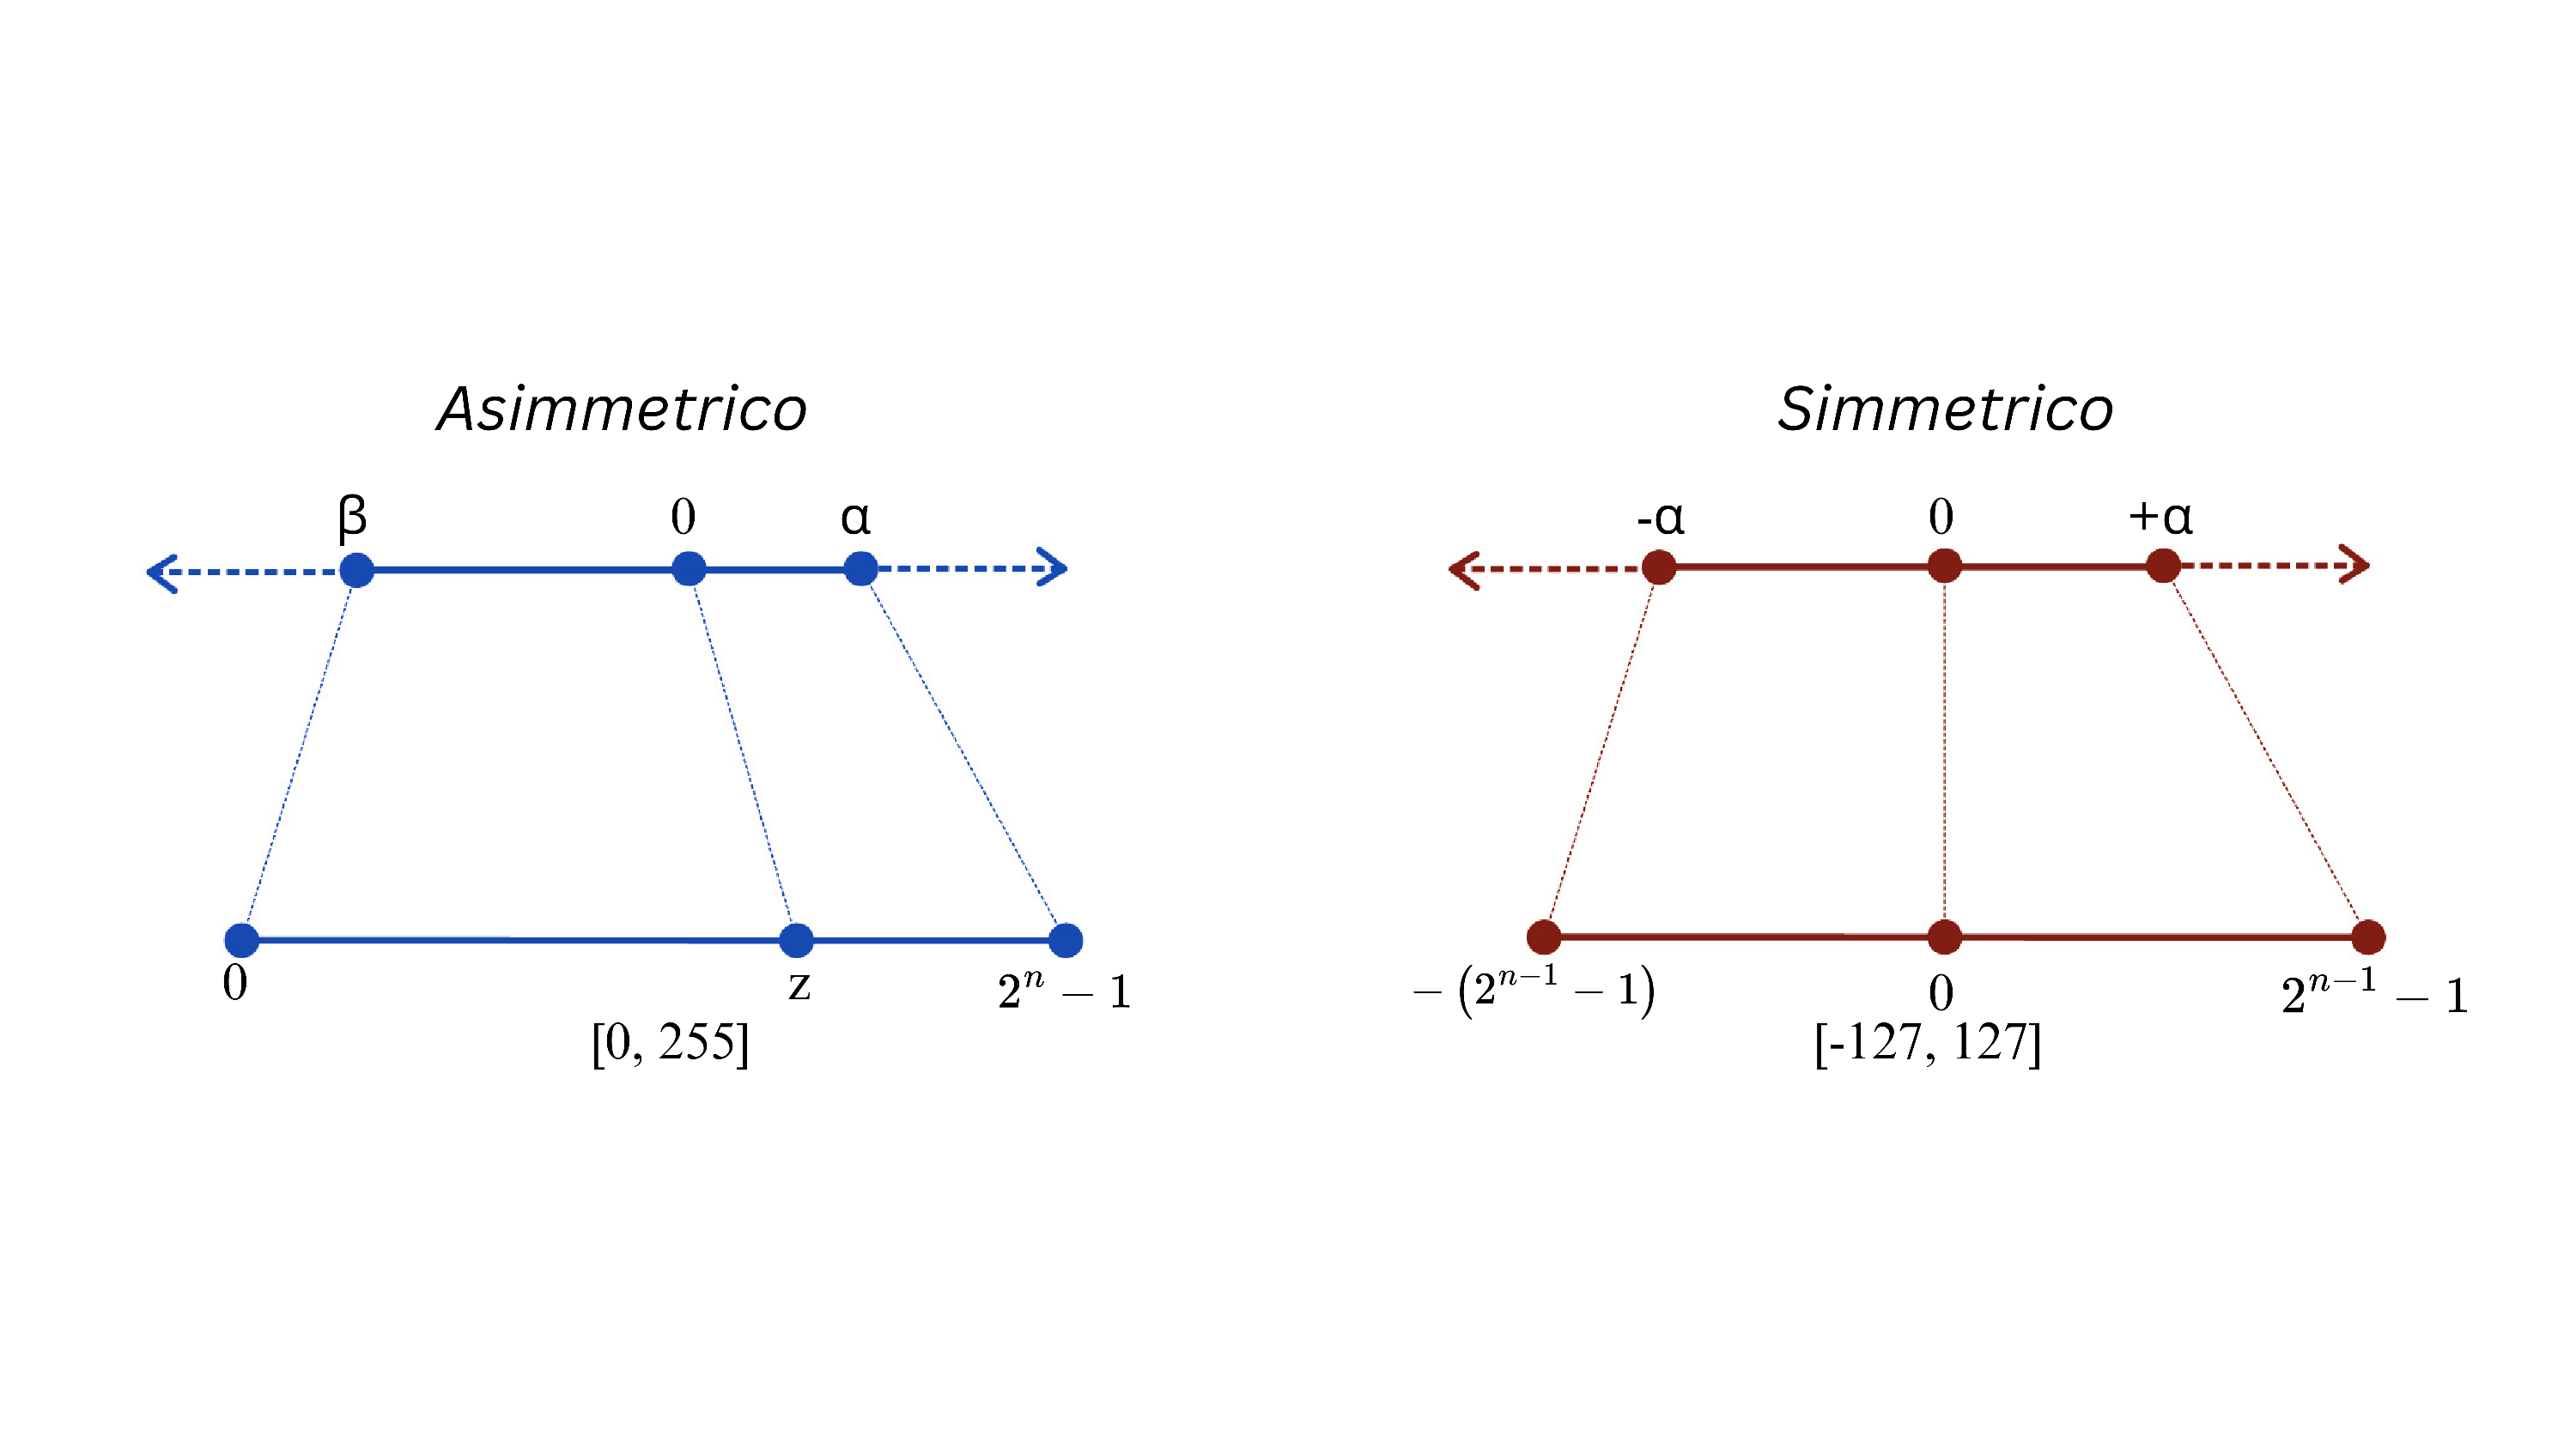
\includegraphics[width=13cm]{img/AsymmetricSymmetric.pdf}
    \caption{Differenza tra tecnica asimmetrica e simmetrica}
    \end{figure}
    \\
    Quantizzazione Asimmetrica:
    \begin{itemize}
        \item \textbf{Scala Non Uniforme}: Nella quantizzazione asimmetrica, i valori del modello vengono mappati in uno spazio quantizzato che non è centrato attorno allo zero. L'intervallo dei valori positivi e negativi è solitamente diverso e dipende da $\alpha$ e $\beta$
        \item \textbf{Range di Quantizzazione}: Viene definito un fattore di scala $s$ diverso per i valori positivi e negativi, o un valore di offset $z$ che permette di gestire l'intervallo in modo più flessibile.
        \item \textbf{Flessibilità Maggiore}: Permette una rappresentazione più precisa per distribuzioni di valori che non sono simmetriche attorno allo zero.
    \end{itemize}
    Per ottenere la quantizzazione asimmetrica, $x_q$ del numero $x_f$ si utilizzano le seguenti formule:
    
    \centerline{$x_q=\operatorname{clamp}\left(\left\lfloor\frac{x_f}{s}\right\rfloor+z ; 0 ; 2^n-1\right) \quad s=\frac{\alpha-\beta}{2^n-1} \quad z=\left\lfloor-1 \times \frac{\beta}{s}\right\rfloor$}
    
    In caso si volesse riconvertire al numero originario il numero quantizzato attraverso la tecnica asimmetrica la formula è la seguente:\\
    \centerline{$x_f = s(x_q-z)$.}
    Quantizzazione Simmetrica:
    \begin{itemize}
        \item \textbf{Scala Uniforme}: Nella quantizzazione simmetrica, i valori del modello vengono mappati in uno spazio quantizzato che è centrato attorno allo 0, sostanzialmente lo 0 quantizzato rimane 0. Ciò significa che l'intervallo dei valori positivi e negativi è uguale.
        \item \textbf{Range di Quantizzazione}: Viene definito un unico fattore di scala $s$ che determina come i valori in virgola mobile vengono convertiti in valori interi. Questo fattore di scala è uguale per i valori positivi e negativi.
        \item  \textbf{Semplicità di Implementazione}: La simmetria attorno allo zero rende più semplici i calcoli e diminuisce l'hardware necessario per la quantizzazione.
    \end{itemize}
    Per ricavare quindi il numero quantizzato $x_q$ è necessario applicare le seguenti formule:
    \centerline{$x_q=\operatorname{clamp}\left(\left\lfloor\frac{x_f}{s}\right\rfloor ;-\left(2^{n-1}-1\right) ; 2^{n-1}-1\right) \quad s=\frac{|\alpha|}{2^{n-1}-1}$}
    Nel caso in cui invece si volesse riconvertire al numero originario il numero quantizzato attraverso la tecnica simmetrica la formula è la seguente:\\
    \centerline{$x_f = sx_q$.}


    % cos'è 
    % a cosa serve
    % cosa si è utilizzato -> quantizzazione di un modello preaddestrato vedi Colab
    \subsubsection{Sviluppo}
    Per la quantizzazione, si è proceduto direttamente quantizzando Phi3-mini. Come visibile in figura 4.4, il modello, che ha subito il fine-tuning, è stato precedentemente quantizzato da 32-bit floating point a 8-bit interi. Questo è stato possibile attraverso il seguente frammento di codice:
    
    \begin{figure}[htp]
    \centering
    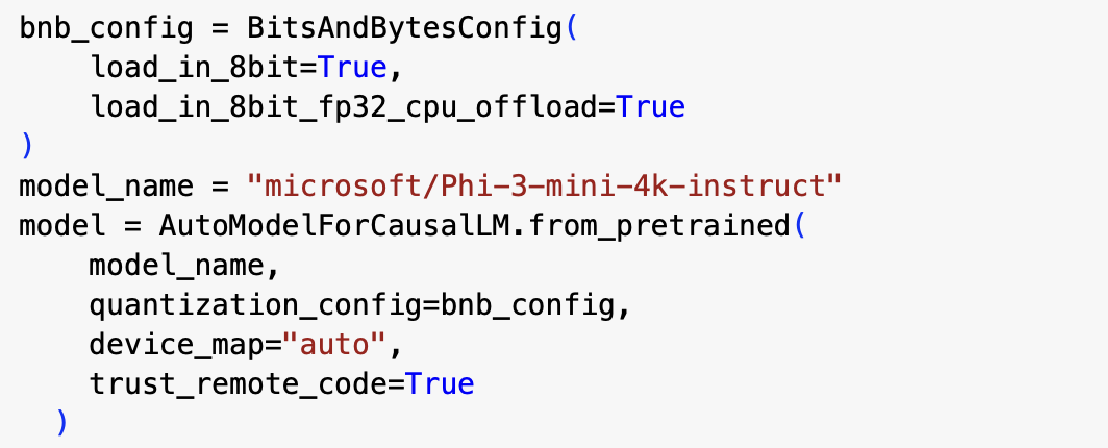
\includegraphics[width=10cm]{img/bitsAndBytes.pdf}
    \caption{Errore relativo asimmetrico suddiviso nei diversi bit di quantizzazione}
    \end{figure}
    In particolare, si è utilizzato il plugin BitsAndBytesConfig, che permette di quantizzare a 8-bit o a 4-bit qualsiasi modello.
    La quantizzazione ha quindi reso possibile una maggiore velocità per l'inferenza e inoltre anche un consumo ridotto delle risorse a disposizione.

    \subsubsection{Test errore di quantizzazione}
     È noto che scalando 32-bit in un numero di bit minore vi sarà sicuramente una perdita, anche minima, di informazione. In seguito è possibile visionare errore relativo in percentuale che deriva dalla quantizzazione.\\
     \centerline{$errore\_relativo = \frac{|x - x_q|}{\DeclarePairedDelimiter{|x|}}$, con $x$ valore a 32-bit, e $x_q$, valore quantizzato,}
     In figura 4.11 e 4.12 è possibile visualizzare in percentuale l'errore relativo asimmetrico e simmetrico rispetto a 1000 valori.
    \begin{figure}[!h]
        \centering        
        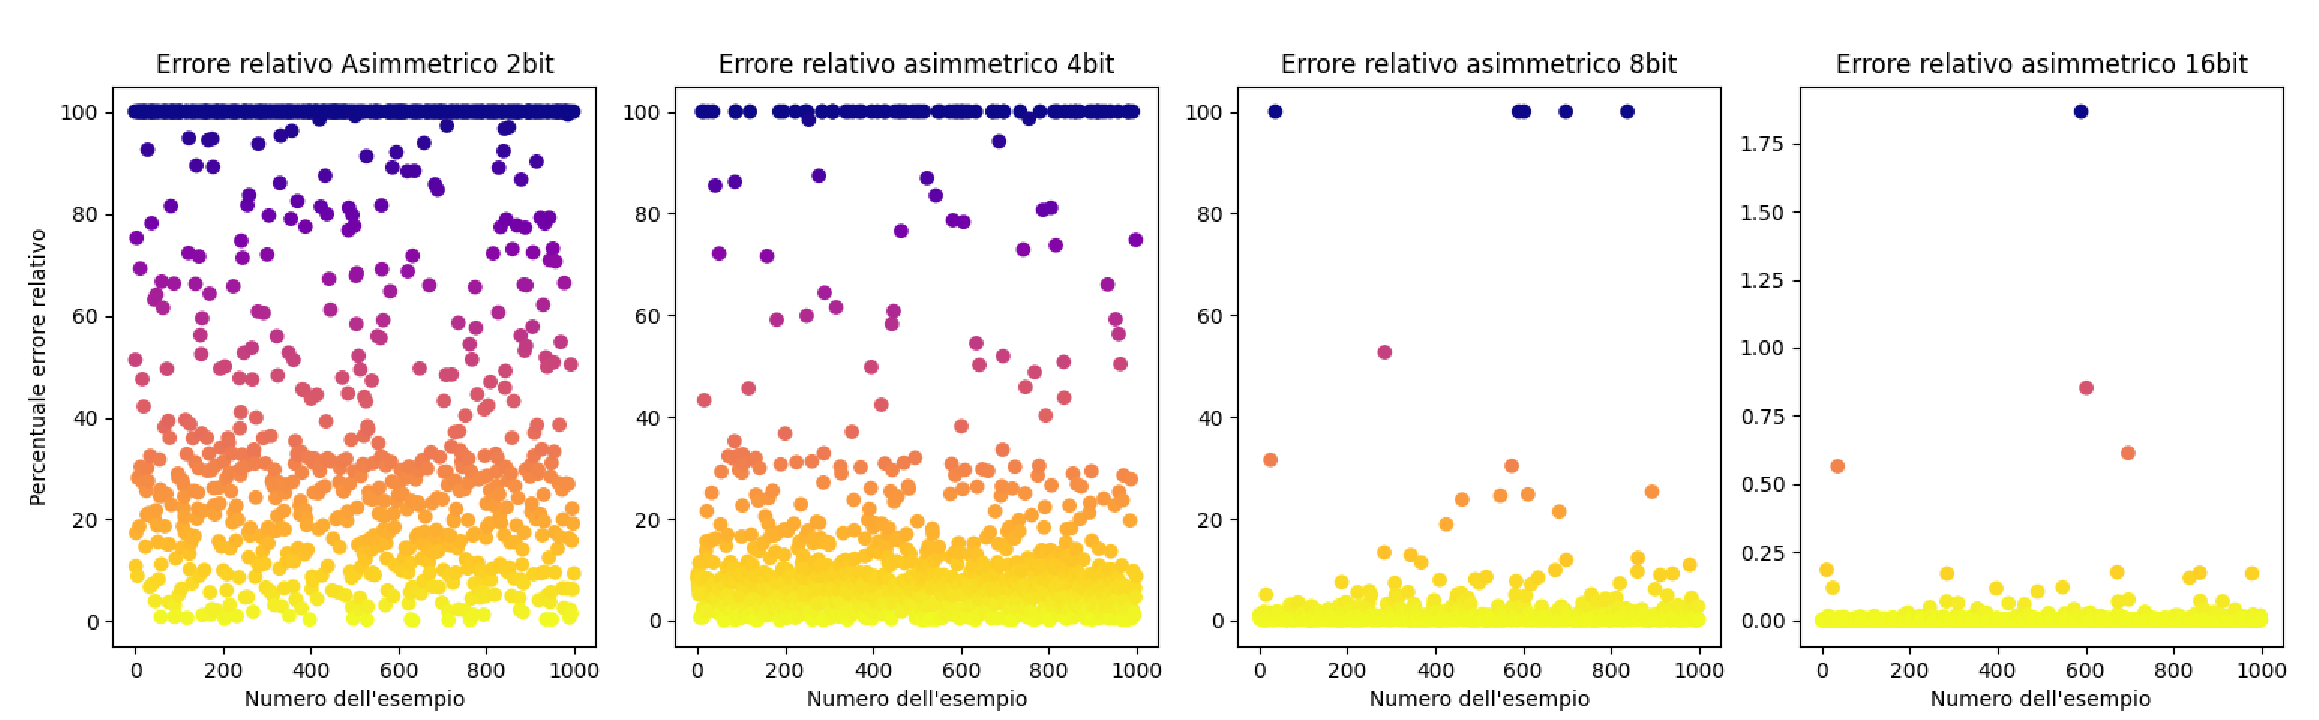
\includegraphics[width=14.5cm]{img/totA.pdf}
        \caption{Errore relativo asimmetrico suddiviso nei diversi bit di quantizzazione}
    \end{figure}\newline
    \begin{figure}[!h]
        \centering        
        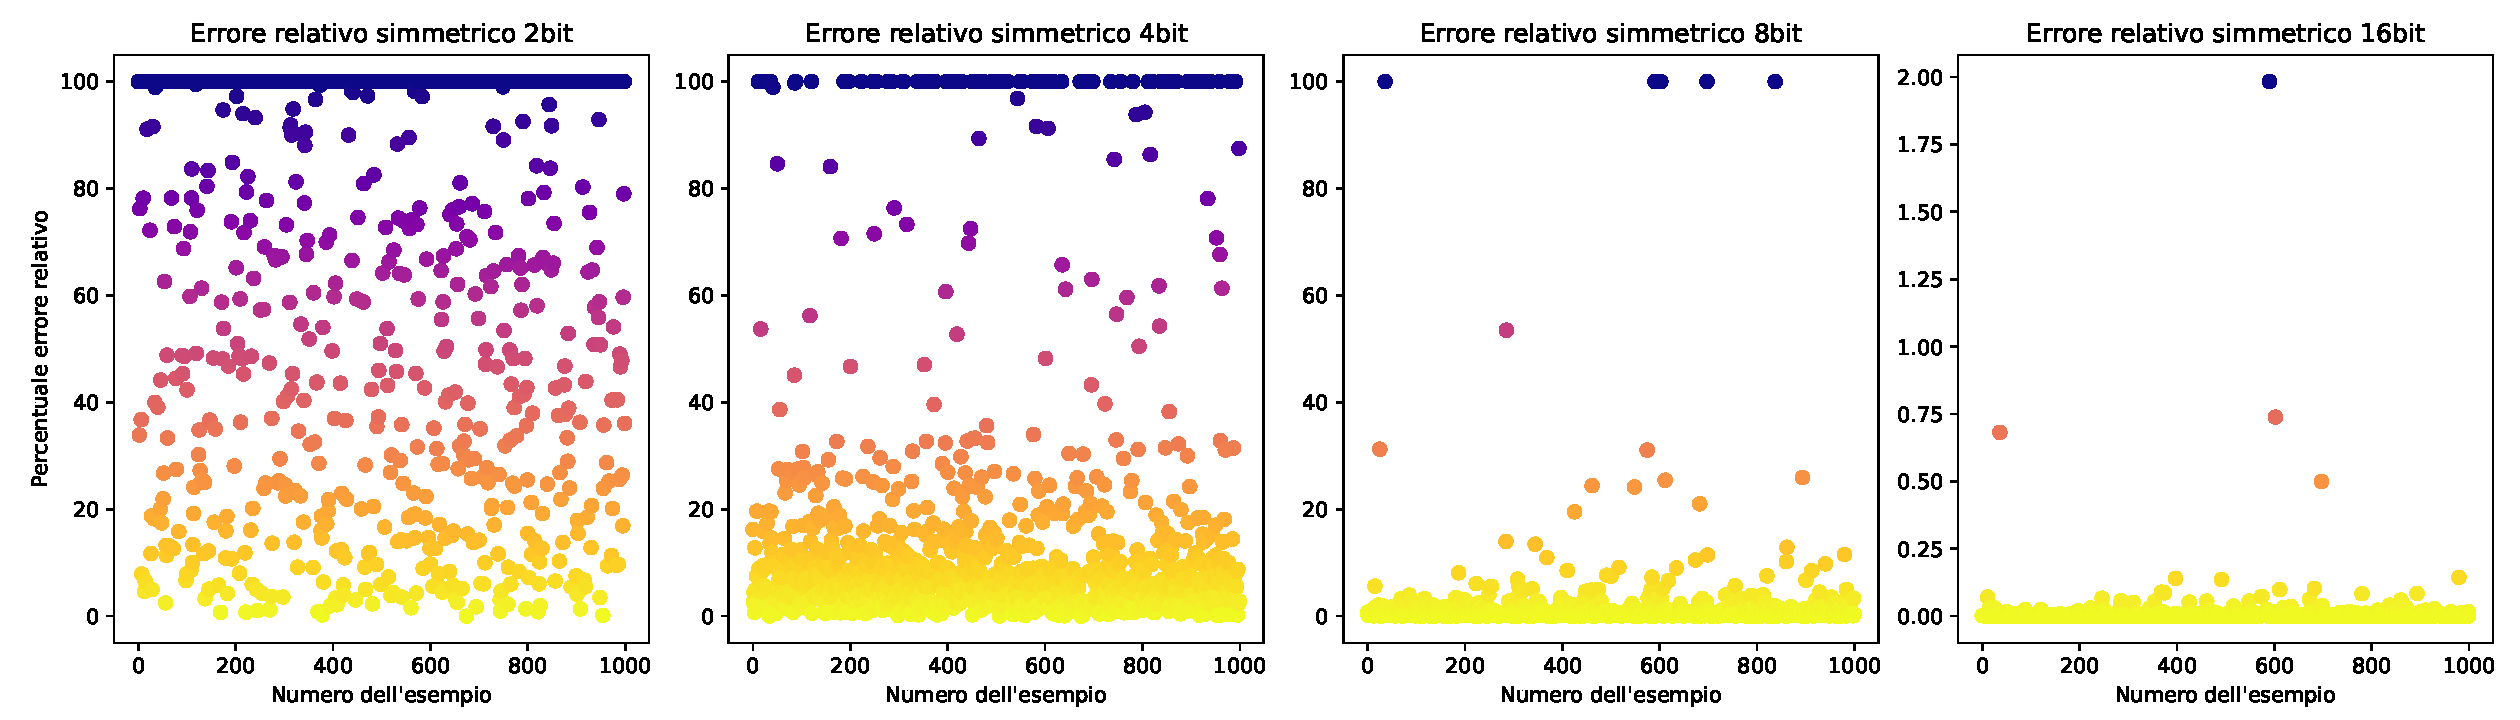
\includegraphics[width=14.5cm]{img/totS.pdf}
        \caption{Errore relativo simmetrico suddiviso nei diversi bit di quantizzazione}
    \end{figure}    
    \newline
    % test su perdita di dati della quantizzazione

    
\section{Resoconto finale}
    \subsection{Prodotti ottenuti}
        %loss function di modelli addestrati con colab e llamacpp
    \subsection{Risultati ottenuti}
        % bene o male, pro e contro del PROGETTO e di come è stato affrontato
        % bene perchè si sono notati risultati
        
        % male perchè costoso 
    \subsection{Conclusione}
    

\newpage
    \chapter{Valutazione retrospettiva}
\label{chap:conclusioni}
    \section{Conoscenze acquisite}
    Durante l’esperienza in Zucchetti, sono stati affrontati diversi temi legati all'intelligenza artificiale. I \textit{test} sono stati il tema principale dello stage; infatti, sebbene le tecniche studiate fossero molto diverse tra loro, l'obiettivo principale era migliorare la generazione di \textit{test}.
    Le conoscenze acquisite sono variate notevolmente tra il primo e il secondo macro periodo. Nel primo periodo, sono state apprese nozioni riguardanti gli \gls{llmse}, che costituiscono la base del lavoro sulla generazione di \textit{test}. È stato particolarmente importante delineare un percorso per futuri approfondimenti; comprendere che i \textit{test} generati sono qualitativamente migliori se il codice è in inglese e il linguaggio è tipizzato è stato di fondamentale importanza.
    Nel secondo macro periodo, invece, le nozioni sono state principalmente legate alla specializzazione del modello tramite \gls{fine-tuning}. Sono state apprese tecniche come \gls{lora} e approfondite alcune delle possibili migliorie applicabili, come \textit{MoLE} e \textit{AdaMoLE}.
    Oltre alla specializzazione del modello, è stata esaminata a fondo la quantizzazione. Sono state approfondite le tecniche di quantizzazione asimmetrica e simmetrica e la loro applicazione agli \gls{llm}, al fine di ridurre le loro dimensioni.    
    Le conoscenze acquisite non si sono limitate all'ambito lavorativo, ma hanno arricchito anche il lato personale. Durante lo stage, sono state infatti molte le lezioni apprese, la maggior parte delle quali deriva dall'interazione con i colleghi e il responsabile dello stage, Gregorio Piccoli. Queste esperienze hanno contribuito significativamente alla crescita professionale e personale.
        %cosa ho imparato dallo stage
    \section{Valutazione personale}
            %cosa ho fatto bene -> rispetto obiettivi, integrazione col team
    La valutazione che può essere associata con l'esperienza trascorsa durante questo stage è sicuramente più che positiva.
    Durante il percorso è stato appreso come gestire un progetto in un ambiente di lavoro professionale e innovativo, ricercando efficacia, efficienza e qualità in ciò che doveva essere completato.
    È stato inoltre significativo affacciarsi al mondo della ricerca e sviluppo all'interno di una grande azienda come Zucchetti, poiché rappresenta un segmento molto interessante e dinamico. Questa esperienza ha permesso di comprendere meglio le dinamiche e le sfide legate all'innovazione tecnologica in un contesto aziendale di alto livello.
    Un'ulteriore prova del successo dello stage deriva dal rapporto personale che si è creato con i colleghi. Questo aspetto è di grande rilevanza poiché favorisce il confronto e il miglioramento delle capacità comunicative.
        %cosa avrei potuto fare meglio 
    Non vi sono solo ovviamente solo obiettivi raggiunti e rapporti instaurati, durante un primo incontro con la vita lavorativa all'interno di un'azienda sono emerse anche difficoltà. 
     La principale difficoltà è stata mantenere costanza e dedizione per raggiungere gli obiettivi prefissati, un aspetto spesso sottovalutato.
     Inoltre, sebbene il clima fosse disteso vi è stata la necessità costante di portare risultati di valore con il proprio operato, un aspetto che durante la vita universitaria spesso non si affronta.
    È importante sottolineare che sono state proprio queste piccole difficoltà che hanno accompagnato l'esperienza di stage ad accrescere l'interesse verso lo stage stesso, ponendo ogni giorno un nuovo obiettivo stimolante al fine di migliorare.

\newpage

    \pagenumbering{roman}
    \backmatter
    \chapter{Bibliografia}
\label{cap:bibliography}

\nocite{*}

% Books bibliography
\printbibliography[heading=subbibliography, title={Testi}, type=book]

% Articles bibliography
\printbibliography[heading=subbibliography, title={Articoli}, type=article]

% Websites bibliography
%\printbibliography[heading=subbibliography, title={Siti}, type=online]
    \chapter{Sitografia}
\label{cap:webliography}
\nocite{*}

% Websites bibliography
\printbibliography[heading=subbibliography, title={\null}, type=online]

    \printglossary[type=\acronymtype, title=Acronimi e abbreviazioni, toctitle=Acronimi e abbreviazioni]
    \printglossary[type=main, title=Glossario, toctitle=Glossario]
\end{document}